% Options for packages loaded elsewhere
% Options for packages loaded elsewhere
\PassOptionsToPackage{unicode}{hyperref}
\PassOptionsToPackage{hyphens}{url}
%
\documentclass[
  ignorenonframetext,
  italian,
  compress, aspectratio=149]{beamer}
\newif\ifbibliography
\usepackage{pgfpages}
\setbeamertemplate{caption}[numbered]
\setbeamertemplate{caption label separator}{: }
\setbeamercolor{caption name}{fg=normal text.fg}
\beamertemplatenavigationsymbolshorizontal
% remove section numbering
\setbeamertemplate{part page}{
  \centering
  \begin{beamercolorbox}[sep=16pt,center]{part title}
    \usebeamerfont{part title}\insertpart\par
  \end{beamercolorbox}
}
\setbeamertemplate{section page}{
  \centering
  \begin{beamercolorbox}[sep=12pt,center]{section title}
    \usebeamerfont{section title}\insertsection\par
  \end{beamercolorbox}
}
\setbeamertemplate{subsection page}{
  \centering
  \begin{beamercolorbox}[sep=8pt,center]{subsection title}
    \usebeamerfont{subsection title}\insertsubsection\par
  \end{beamercolorbox}
}
% Prevent slide breaks in the middle of a paragraph
\widowpenalties 1 10000
\raggedbottom
\AtBeginPart{
  \frame{\partpage}
}
\AtBeginSection{
  \ifbibliography
  \else
    \frame{\sectionpage}
  \fi
}
\AtBeginSubsection{
  \frame{\subsectionpage}
}
\usepackage{iftex}
\ifPDFTeX
  \usepackage[T1]{fontenc}
  \usepackage[utf8]{inputenc}
  \usepackage{textcomp} % provide euro and other symbols
\else % if luatex or xetex
  \usepackage{unicode-math} % this also loads fontspec
  \defaultfontfeatures{Scale=MatchLowercase}
  \defaultfontfeatures[\rmfamily]{Ligatures=TeX,Scale=1}
\fi
\usepackage{lmodern}

\usetheme[]{Montpellier}
\usecolortheme[]{dove}
\useinnertheme[]{rounded}
\useoutertheme[]{miniframes}
\ifPDFTeX\else
  % xetex/luatex font selection
\fi
% Use upquote if available, for straight quotes in verbatim environments
\IfFileExists{upquote.sty}{\usepackage{upquote}}{}
\IfFileExists{microtype.sty}{% use microtype if available
  \usepackage[]{microtype}
  \UseMicrotypeSet[protrusion]{basicmath} % disable protrusion for tt fonts
}{}
\makeatletter
\@ifundefined{KOMAClassName}{% if non-KOMA class
  \IfFileExists{parskip.sty}{%
    \usepackage{parskip}
  }{% else
    \setlength{\parindent}{0pt}
    \setlength{\parskip}{6pt plus 2pt minus 1pt}}
}{% if KOMA class
  \KOMAoptions{parskip=half}}
\makeatother


\usepackage{longtable,booktabs,array}
\usepackage{calc} % for calculating minipage widths
\usepackage{caption}
% Make caption package work with longtable
\makeatletter
\def\fnum@table{\tablename~\thetable}
\makeatother
\usepackage{graphicx}
\makeatletter
\newsavebox\pandoc@box
\newcommand*\pandocbounded[1]{% scales image to fit in text height/width
  \sbox\pandoc@box{#1}%
  \Gscale@div\@tempa{\textheight}{\dimexpr\ht\pandoc@box+\dp\pandoc@box\relax}%
  \Gscale@div\@tempb{\linewidth}{\wd\pandoc@box}%
  \ifdim\@tempb\p@<\@tempa\p@\let\@tempa\@tempb\fi% select the smaller of both
  \ifdim\@tempa\p@<\p@\scalebox{\@tempa}{\usebox\pandoc@box}%
  \else\usebox{\pandoc@box}%
  \fi%
}
% Set default figure placement to htbp
\def\fps@figure{htbp}
\makeatother



\ifLuaTeX
\usepackage[bidi=basic]{babel}
\else
\usepackage[bidi=default]{babel}
\fi
% get rid of language-specific shorthands (see #6817):
\let\LanguageShortHands\languageshorthands
\def\languageshorthands#1{}


\setlength{\emergencystretch}{3em} % prevent overfull lines

\providecommand{\tightlist}{%
  \setlength{\itemsep}{0pt}\setlength{\parskip}{0pt}}



 


\usepackage{graphicx}
\usepackage{xcolor}
\usepackage{tikz}
\usepackage{multirow}
\newcommand{\cov}{\mathrm{Cov}}
\usetikzlibrary{positioning,shapes,calc,arrows,decorations.pathreplacing}
\AtBeginSubsection{}
\AtBeginDocument{\author[Ottavia M. Epifania]{Ottavia M. Epifania \\ Univeristà di Trento \\\texttt{ottavia.epifania@unitn.it}}}
\AtBeginDocument{\institute[]{A.A. 2026/2027}}
\AtBeginSection[]{
  \begin{frame}[plain]
    \tableofcontents[currentsection,hideallsubsections]
  \end{frame}
}
\AtBeginSubsection[]{
  \begin{frame}[plain]
    \tableofcontents[currentsection,currentsubsection,hideothersubsections]
  \end{frame}
}
\definecolor{unipd}{RGB}{155,0,20}
\definecolor{template}{RGB}{72,79,89}
\definecolor{blu}{rgb}{0.0,0.33,0.71}
\makeatletter
\@ifpackageloaded{tcolorbox}{}{\usepackage[skins,breakable]{tcolorbox}}
\@ifpackageloaded{fontawesome5}{}{\usepackage{fontawesome5}}
\definecolor{quarto-callout-color}{HTML}{909090}
\definecolor{quarto-callout-note-color}{HTML}{0758E5}
\definecolor{quarto-callout-important-color}{HTML}{CC1914}
\definecolor{quarto-callout-warning-color}{HTML}{EB9113}
\definecolor{quarto-callout-tip-color}{HTML}{00A047}
\definecolor{quarto-callout-caution-color}{HTML}{FC5300}
\definecolor{quarto-callout-color-frame}{HTML}{acacac}
\definecolor{quarto-callout-note-color-frame}{HTML}{4582ec}
\definecolor{quarto-callout-important-color-frame}{HTML}{d9534f}
\definecolor{quarto-callout-warning-color-frame}{HTML}{f0ad4e}
\definecolor{quarto-callout-tip-color-frame}{HTML}{02b875}
\definecolor{quarto-callout-caution-color-frame}{HTML}{fd7e14}
\makeatother
\makeatletter
\@ifpackageloaded{caption}{}{\usepackage{caption}}
\AtBeginDocument{%
\ifdefined\contentsname
  \renewcommand*\contentsname{Indice}
\else
  \newcommand\contentsname{Indice}
\fi
\ifdefined\listfigurename
  \renewcommand*\listfigurename{Elenco delle Figure}
\else
  \newcommand\listfigurename{Elenco delle Figure}
\fi
\ifdefined\listtablename
  \renewcommand*\listtablename{Elenco delle Tabelle}
\else
  \newcommand\listtablename{Elenco delle Tabelle}
\fi
\ifdefined\figurename
  \renewcommand*\figurename{Figura}
\else
  \newcommand\figurename{Figura}
\fi
\ifdefined\tablename
  \renewcommand*\tablename{Tabella}
\else
  \newcommand\tablename{Tabella}
\fi
}
\@ifpackageloaded{float}{}{\usepackage{float}}
\floatstyle{ruled}
\@ifundefined{c@chapter}{\newfloat{codelisting}{h}{lop}}{\newfloat{codelisting}{h}{lop}[chapter]}
\floatname{codelisting}{Lista}
\newcommand*\listoflistings{\listof{codelisting}{Elenco degli Elenchi}}
\makeatother
\makeatletter
\makeatother
\makeatletter
\@ifpackageloaded{caption}{}{\usepackage{caption}}
\@ifpackageloaded{subcaption}{}{\usepackage{subcaption}}
\makeatother

\usepackage{bookmark}
\IfFileExists{xurl.sty}{\usepackage{xurl}}{} % add URL line breaks if available
\urlstyle{same}
\hypersetup{
  pdftitle={Modulo Didattico 4: Principali distribuzioni di probabilità},
  pdfauthor={Ottavia M. Epifania},
  pdflang={it},
  hidelinks,
  pdfcreator={LaTeX via pandoc}}


\title{Modulo Didattico 4: Principali distribuzioni di probabilità}
\subtitle{Corso Analisi dei dati con applicazioni informatiche}
\author{Ottavia M. Epifania}
\date{}

\begin{document}
\frame{\titlepage}


\section{Funzioni di probabilità
discrete}\label{funzioni-di-probabilituxe0-discrete}

\subsection{Definizioni generali}\label{definizioni-generali}

\begin{frame}{}
\phantomsection\label{section}
Sia \(X\) una variabile casuale discreta che assume valori in un insieme
numerabile \(S \subset \mathbb{R}\). La \emph{funzione di probabilità
(massa)} di \(X\) è indicata con \(f_X(x|\theta)\) e definita come:

\[f_X(x|\theta) = \Pr[X = x], \qquad \forall x \in S,\]

al contrario \(f_X(x|\theta) = 0\) per tutti gli \(x \notin S\). In
generale noi considereremo funzioni \(f_X\) parametriche con parametri
\(\theta \in \Theta\):

\[f_X : \mathbb{R} \times \Theta \to [0,1].
\]
\end{frame}

\begin{frame}{Distribuzione di probabilità binomiale}
\phantomsection\label{distribuzione-di-probabilituxe0-binomiale}
\[f_X(x|\theta) = \binom{n}{x}\, \theta^x (1-\theta)^{\,n-x}, 
\qquad x = 0,1,\ldots,n,\]

dove \(\theta \in [0,1]\).

\(\binom{n}{x} = \dfrac{n!}{x!(n-x)!}\) e \[n! =
\begin{cases} 
1 & \text{se } n = 0, \\[2mm]
n \cdot (n-1) \cdot (n-2) \cdots 2 \cdot 1 & \text{se } n > 0.
\end{cases}\]
\end{frame}

\begin{frame}{}
\phantomsection\label{section-1}
\begin{figure}

\begin{minipage}{0.33\linewidth}

\begin{figure}[H]

{\centering \pandocbounded{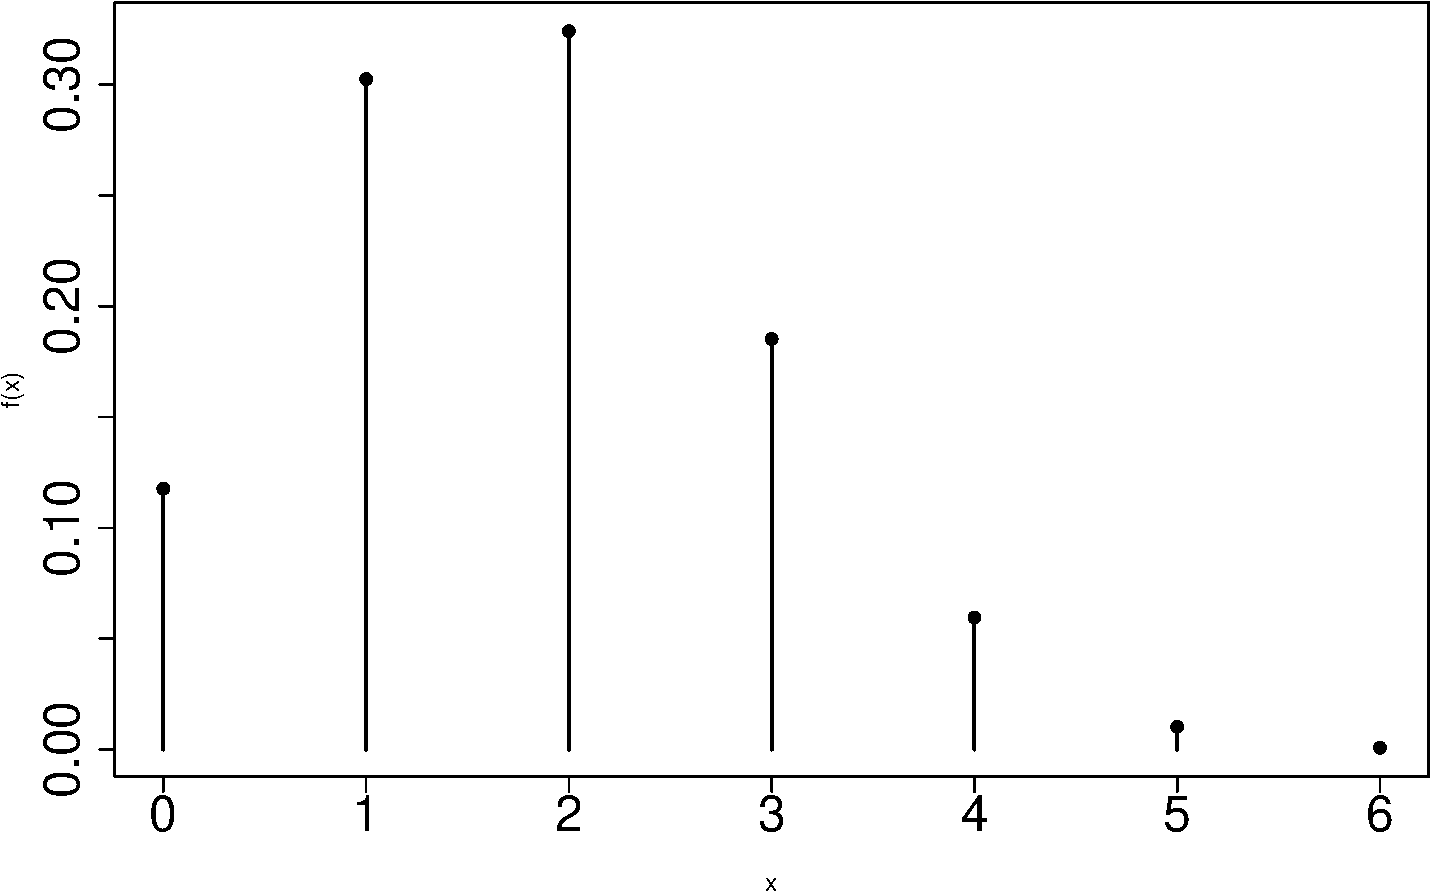
\includegraphics[keepaspectratio]{modulo4_files/figure-beamer/unnamed-chunk-1-1.pdf}}

}

\subcaption{\(\theta = .30\)}

\end{figure}%

\end{minipage}%
%
\begin{minipage}{0.33\linewidth}

\begin{figure}[H]

{\centering \pandocbounded{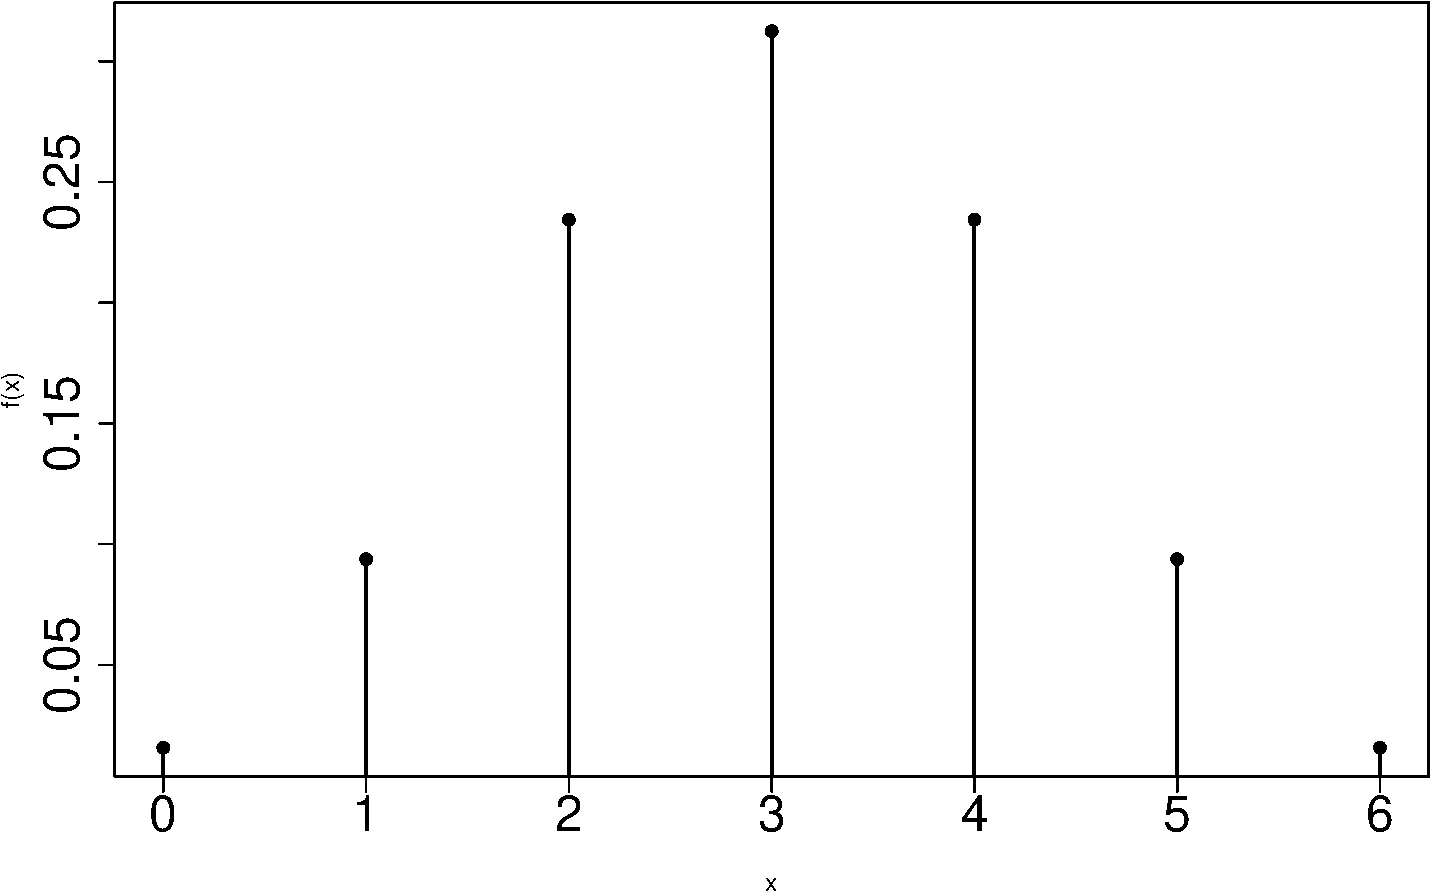
\includegraphics[keepaspectratio]{modulo4_files/figure-beamer/unnamed-chunk-1-2.pdf}}

}

\subcaption{\(\theta = .50\)}

\end{figure}%

\end{minipage}%
%
\begin{minipage}{0.33\linewidth}

\begin{figure}[H]

{\centering \pandocbounded{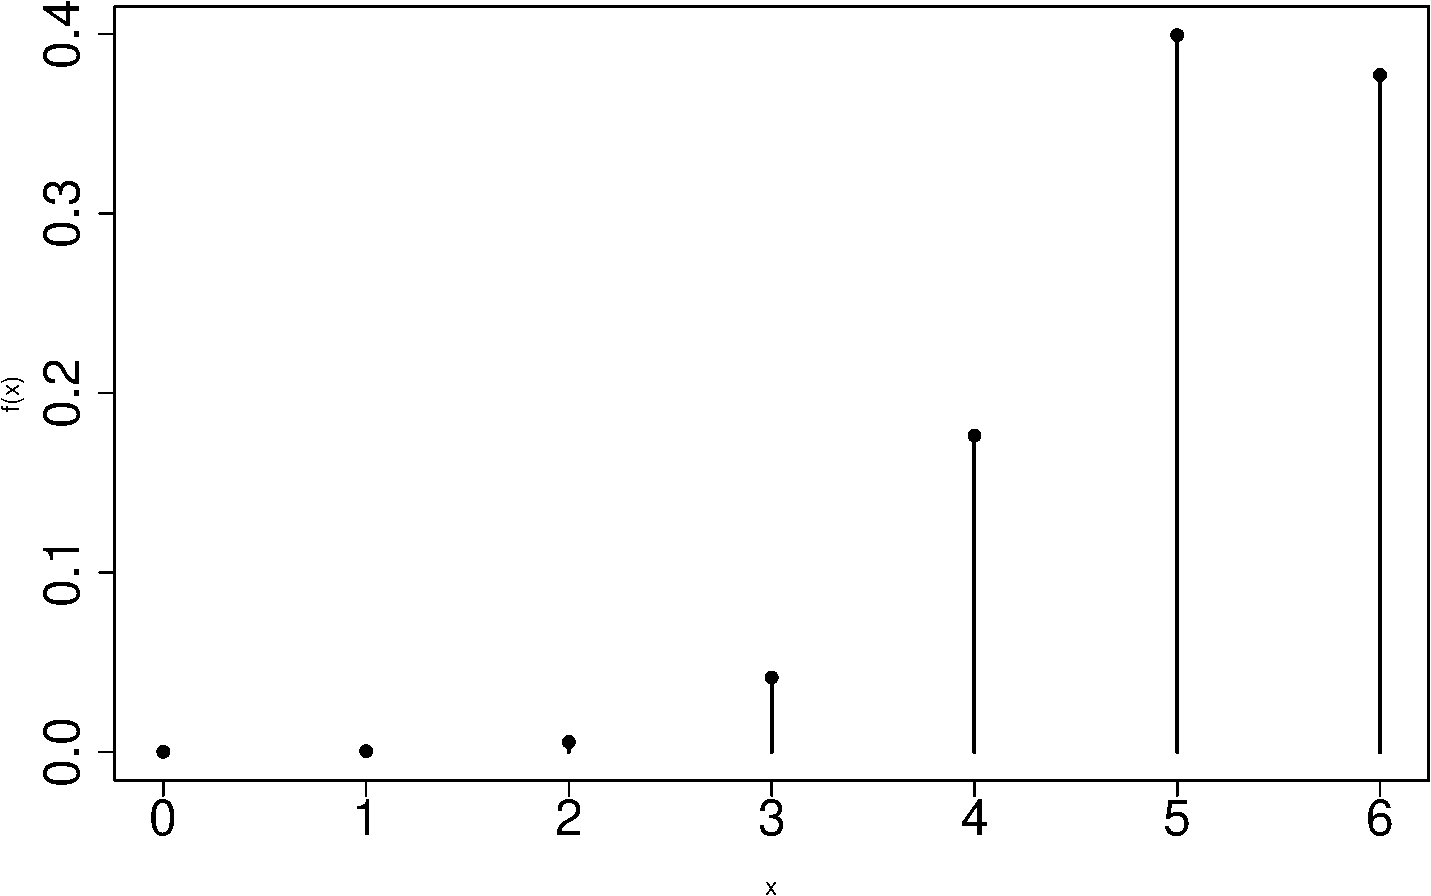
\includegraphics[keepaspectratio]{modulo4_files/figure-beamer/unnamed-chunk-1-3.pdf}}

}

\subcaption{\(\theta = .85\)}

\end{figure}%

\end{minipage}%
\newline
\begin{minipage}{0.33\linewidth}
Massa distribuzione binomiale con
\(S = \{0,1, \ldots, 6 \}\)\end{minipage}%

\end{figure}%
\end{frame}

\begin{frame}{}
\phantomsection\label{section-2}
\begin{figure}

\begin{minipage}{0.33\linewidth}

\begin{figure}[H]

{\centering \pandocbounded{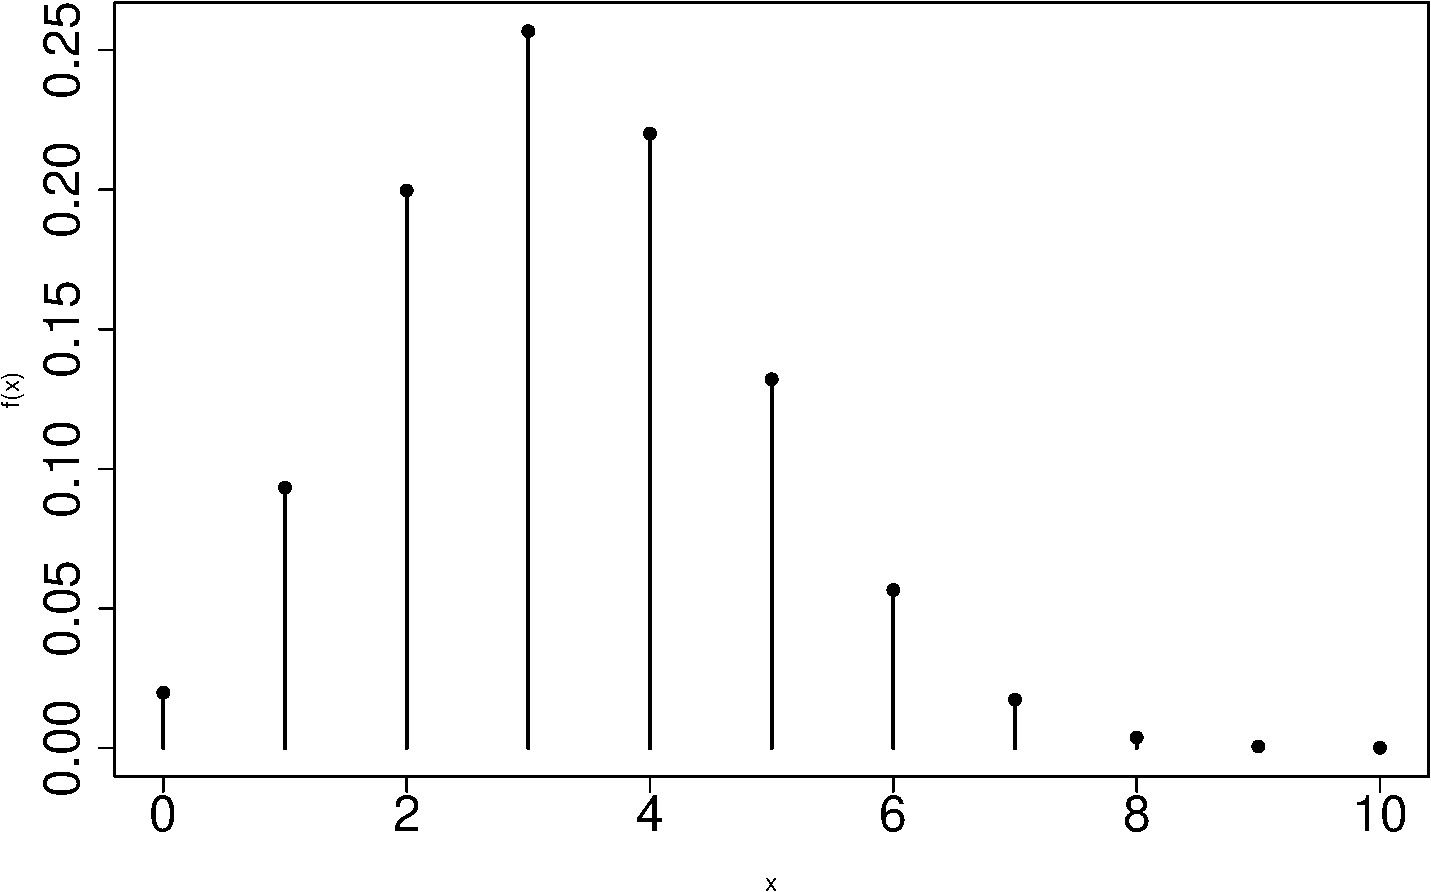
\includegraphics[keepaspectratio]{modulo4_files/figure-beamer/unnamed-chunk-2-1.pdf}}

}

\subcaption{\(\theta = .30\)}

\end{figure}%

\end{minipage}%
%
\begin{minipage}{0.33\linewidth}

\begin{figure}[H]

{\centering \pandocbounded{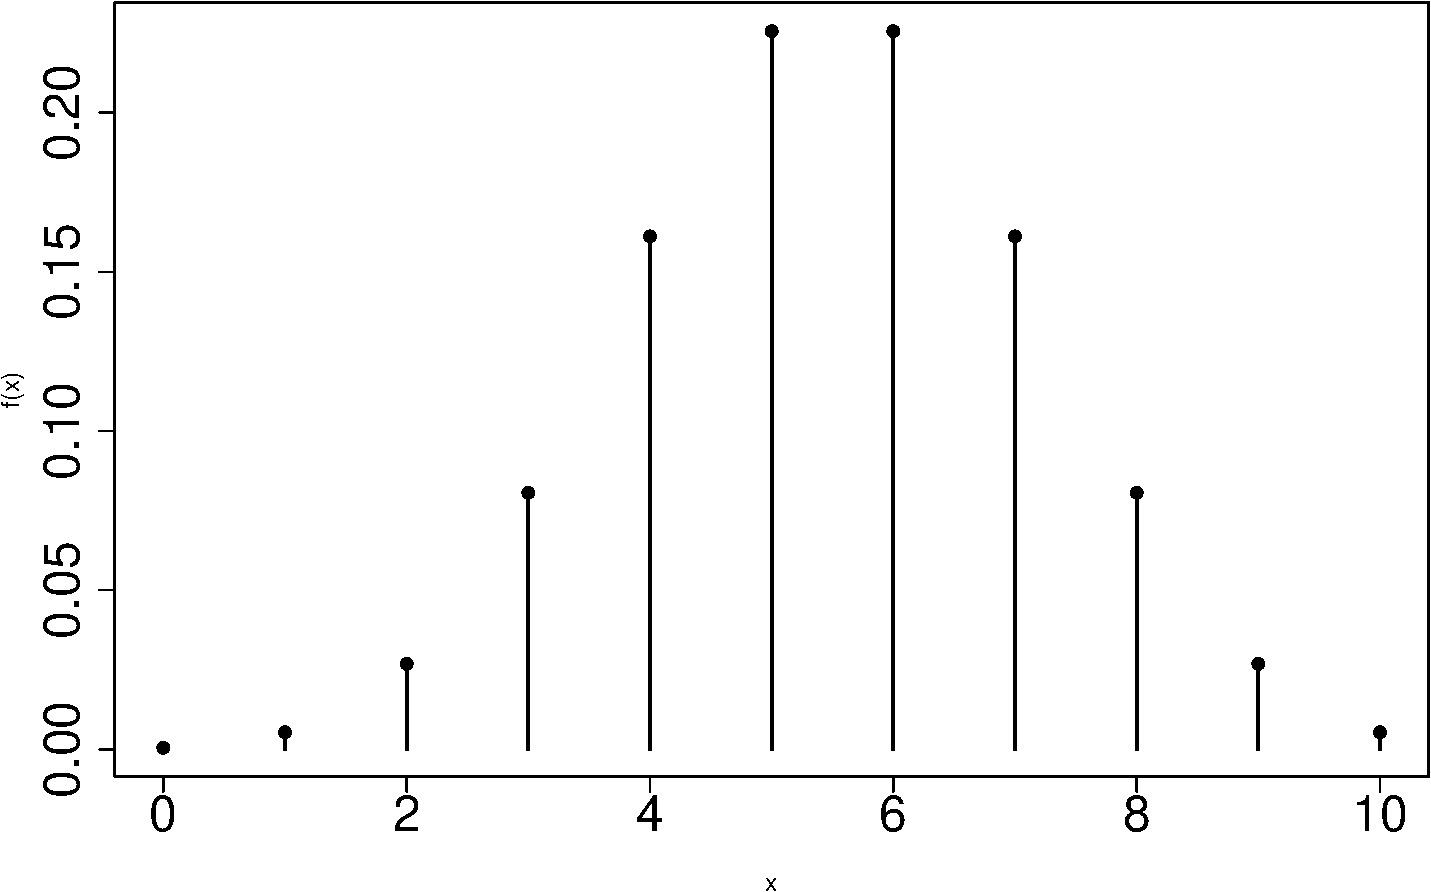
\includegraphics[keepaspectratio]{modulo4_files/figure-beamer/unnamed-chunk-2-2.pdf}}

}

\subcaption{\(\theta = .50\)}

\end{figure}%

\end{minipage}%
%
\begin{minipage}{0.33\linewidth}

\begin{figure}[H]

{\centering \pandocbounded{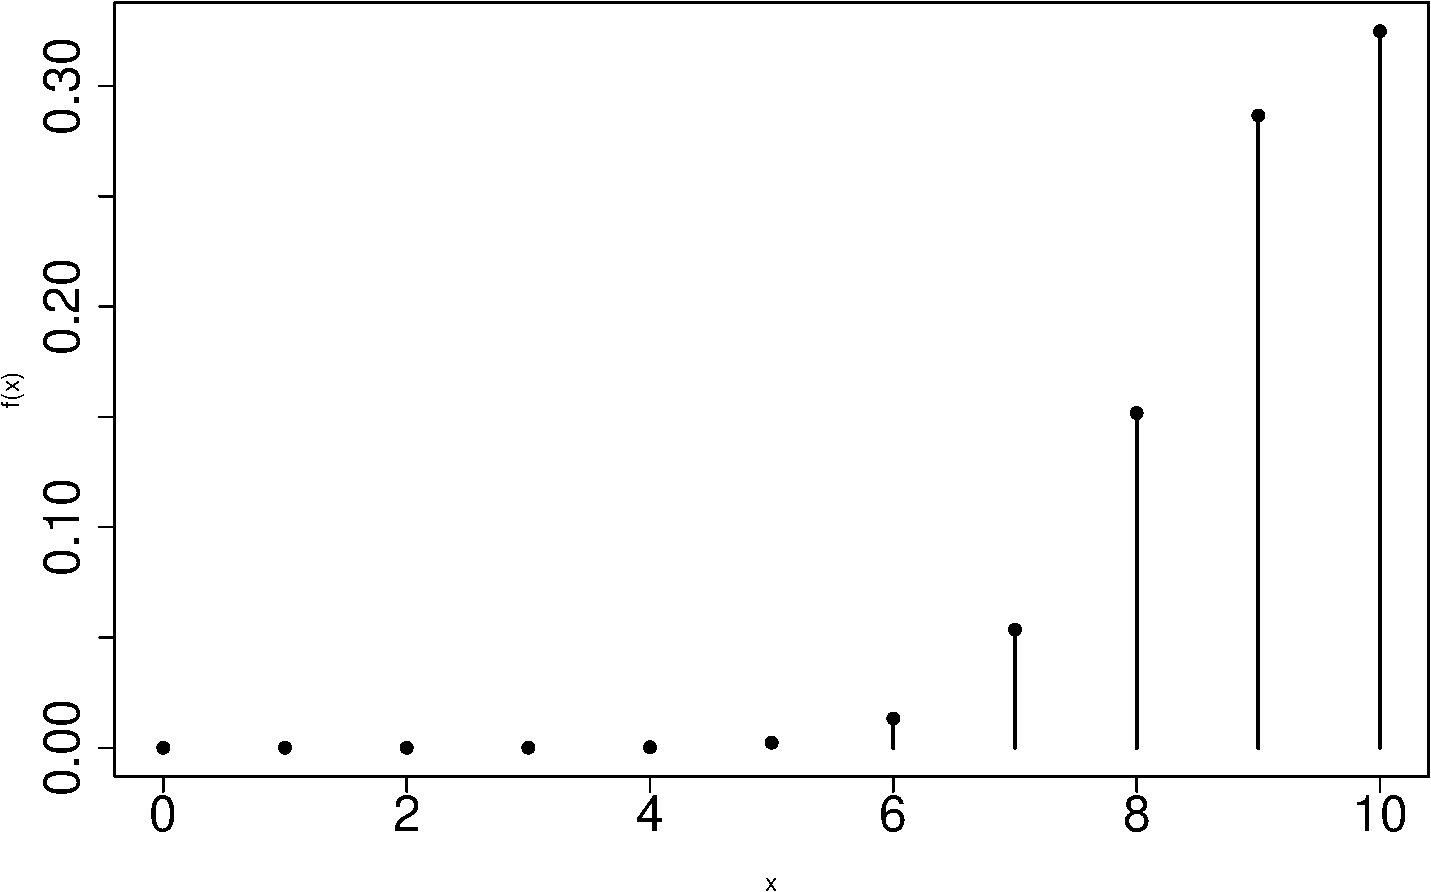
\includegraphics[keepaspectratio]{modulo4_files/figure-beamer/unnamed-chunk-2-3.pdf}}

}

\subcaption{\(\theta = .85\)}

\end{figure}%

\end{minipage}%
\newline
\begin{minipage}{0.33\linewidth}
Massa distribuzione binomiale con
\(S = \{0,1, \ldots, 10 \}\)\end{minipage}%

\end{figure}%
\end{frame}

\begin{frame}{}
\phantomsection\label{section-3}
\begin{figure}

\begin{minipage}{0.33\linewidth}

\begin{figure}[H]

{\centering \pandocbounded{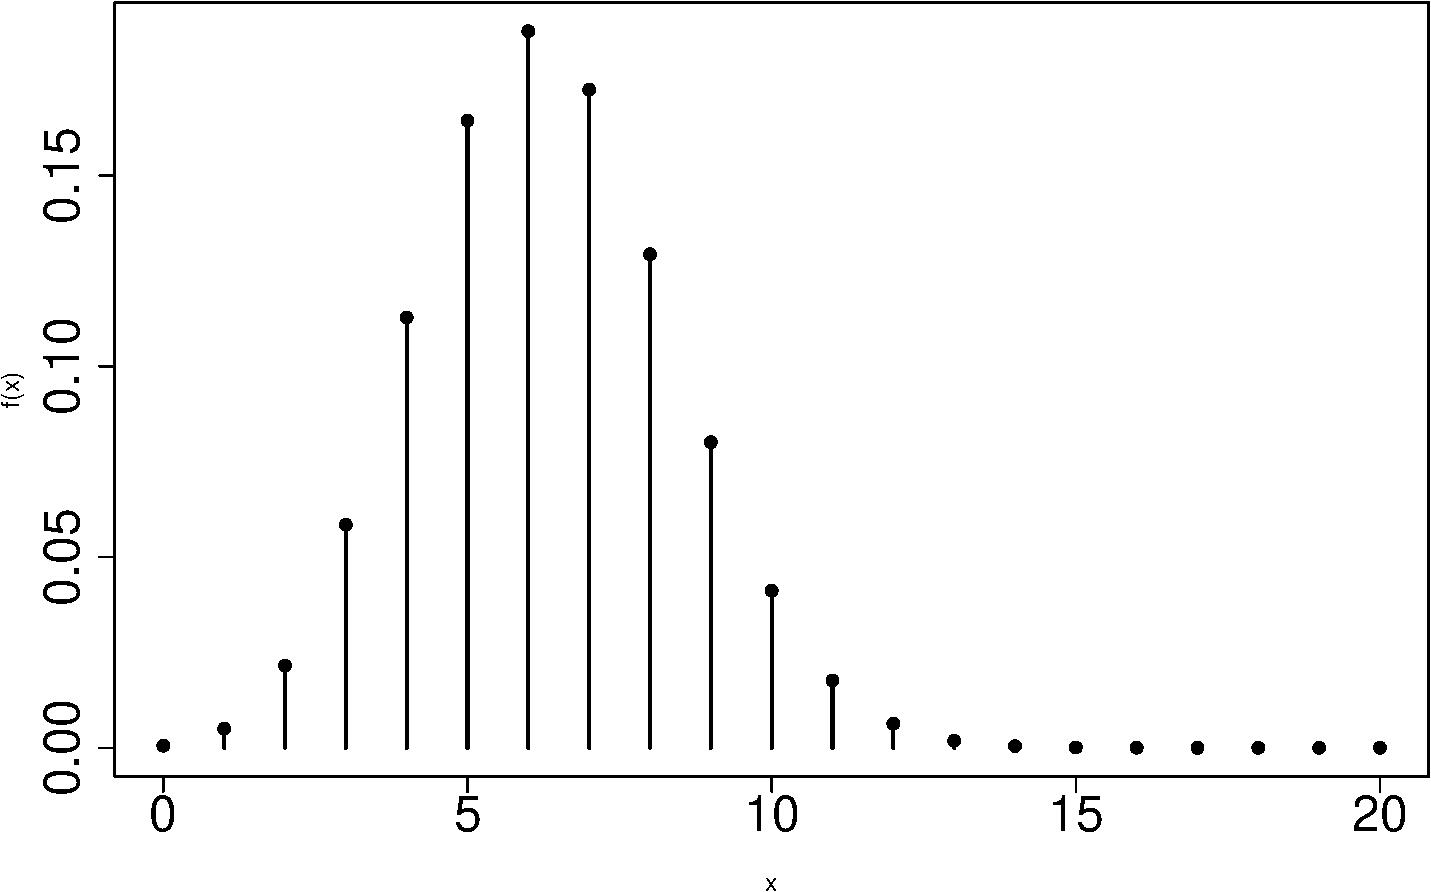
\includegraphics[keepaspectratio]{modulo4_files/figure-beamer/unnamed-chunk-3-1.pdf}}

}

\subcaption{\(\theta = .30\)}

\end{figure}%

\end{minipage}%
%
\begin{minipage}{0.33\linewidth}

\begin{figure}[H]

{\centering \pandocbounded{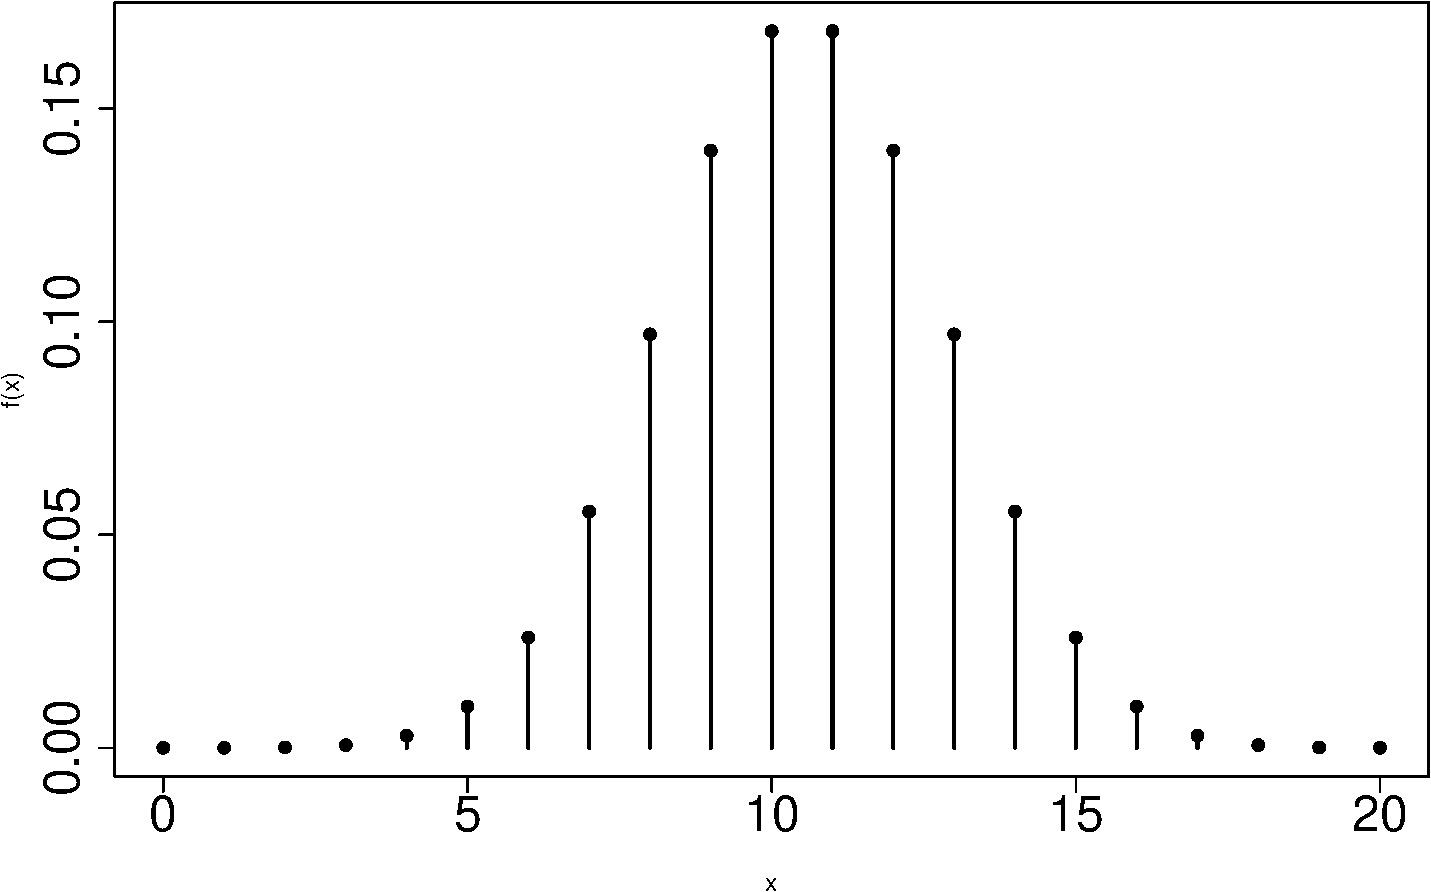
\includegraphics[keepaspectratio]{modulo4_files/figure-beamer/unnamed-chunk-3-2.pdf}}

}

\subcaption{\(\theta = .50\)}

\end{figure}%

\end{minipage}%
%
\begin{minipage}{0.33\linewidth}

\begin{figure}[H]

{\centering \pandocbounded{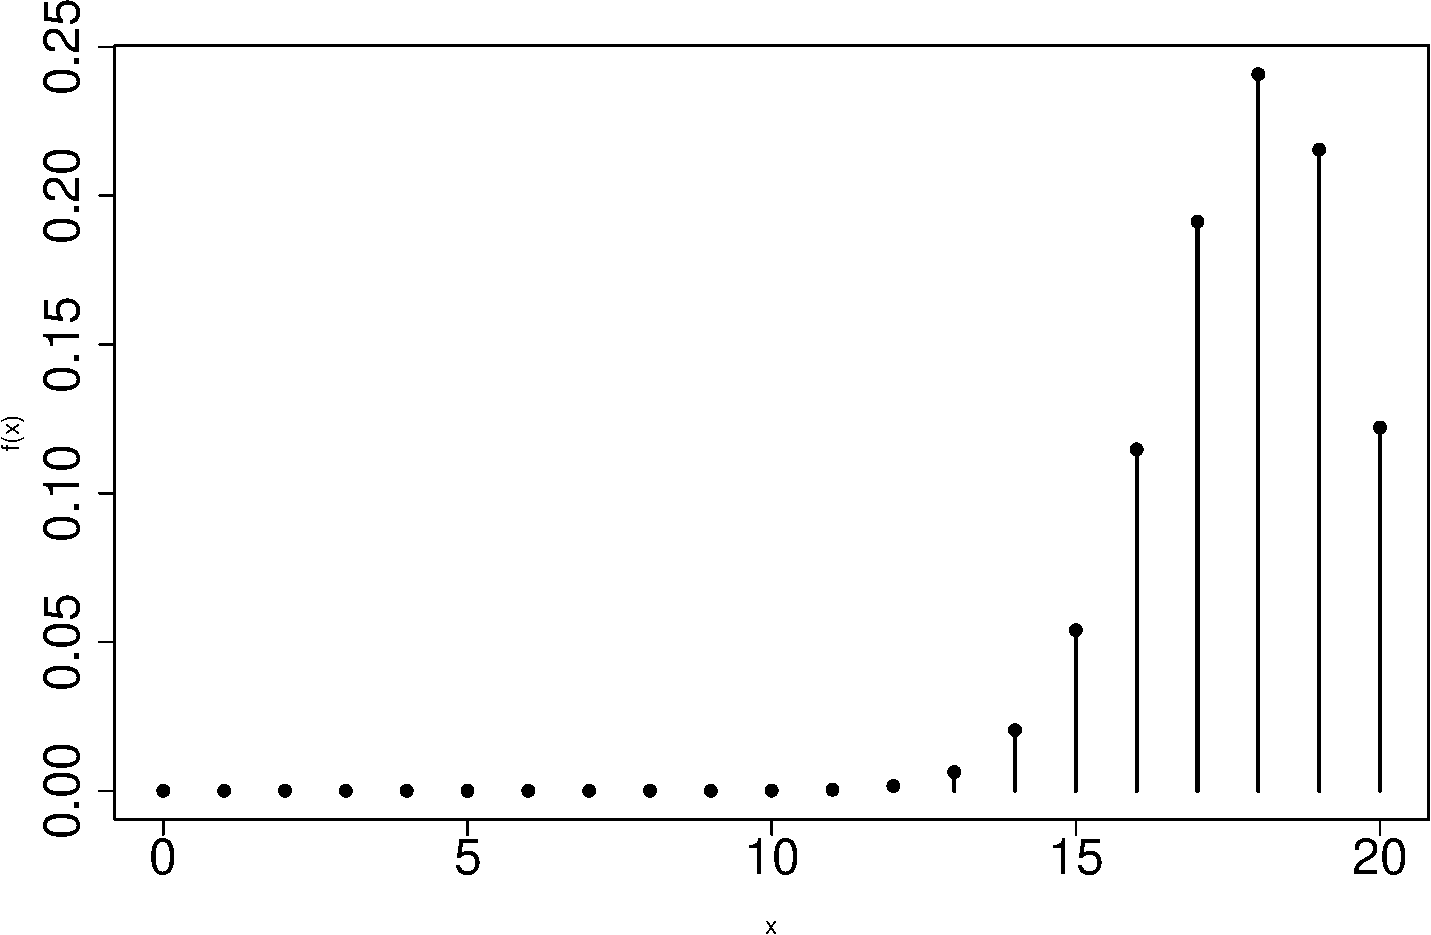
\includegraphics[keepaspectratio]{modulo4_files/figure-beamer/unnamed-chunk-3-3.pdf}}

}

\subcaption{\(\theta = .85\)}

\end{figure}%

\end{minipage}%
\newline
\begin{minipage}{0.33\linewidth}
Massa distribuzione binomiale con
\(S = \{0,1, \ldots, 20 \}\)\end{minipage}%

\end{figure}%
\end{frame}

\begin{frame}{}
\phantomsection\label{section-4}
La \emph{funzione di probabilità cumulata} di una variabile casuale
discreta \(X\) si indica con \(F_X(x|\theta)\) ed è definita come:

\[F_X(x|\theta) = \Pr[X \leq x]
= \sum_{s \in S: \, s \leq x} f_X(s).\]

In altre parole, \(F_X(x|\theta)\) rappresenta la probabilità che \(X\)
assuma un valore minore o uguale a \(x\).\\
Chiaramente, \[F_X : \mathbb{R} \times \Theta \longrightarrow [0,1].\]
\end{frame}

\begin{frame}{Distribuzione binomiale cumulata}
\phantomsection\label{distribuzione-binomiale-cumulata}
Se \(X \sim \text{Bin}(n,\theta)\), allora la funzione di probabilità
cumulata è:

\[F_X(x|\theta) = \sum_{z=0}^{x} \binom{n}{z}\, \theta^z (1-\theta)^{\,n-z}, 
\qquad x = 0,1,\ldots,n,\]

dove \(\theta \in [0,1]\).
\end{frame}

\begin{frame}{}
\phantomsection\label{section-5}
\begin{figure}

\begin{minipage}{0.33\linewidth}

\begin{figure}[H]

{\centering \pandocbounded{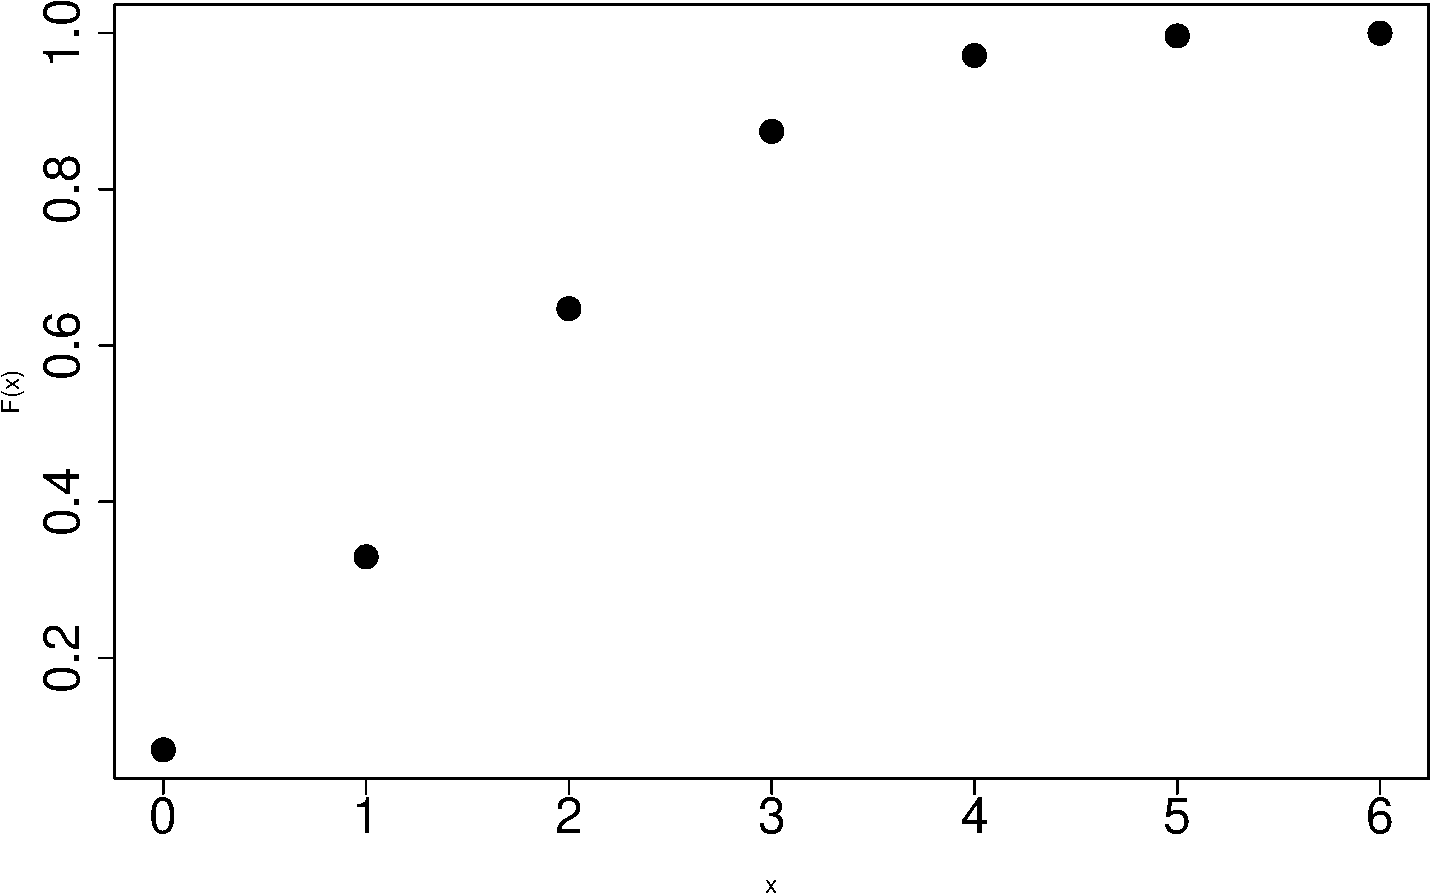
\includegraphics[keepaspectratio]{modulo4_files/figure-beamer/unnamed-chunk-4-1.pdf}}

}

\subcaption{\(\theta = .30\)}

\end{figure}%

\end{minipage}%
%
\begin{minipage}{0.33\linewidth}

\begin{figure}[H]

{\centering \pandocbounded{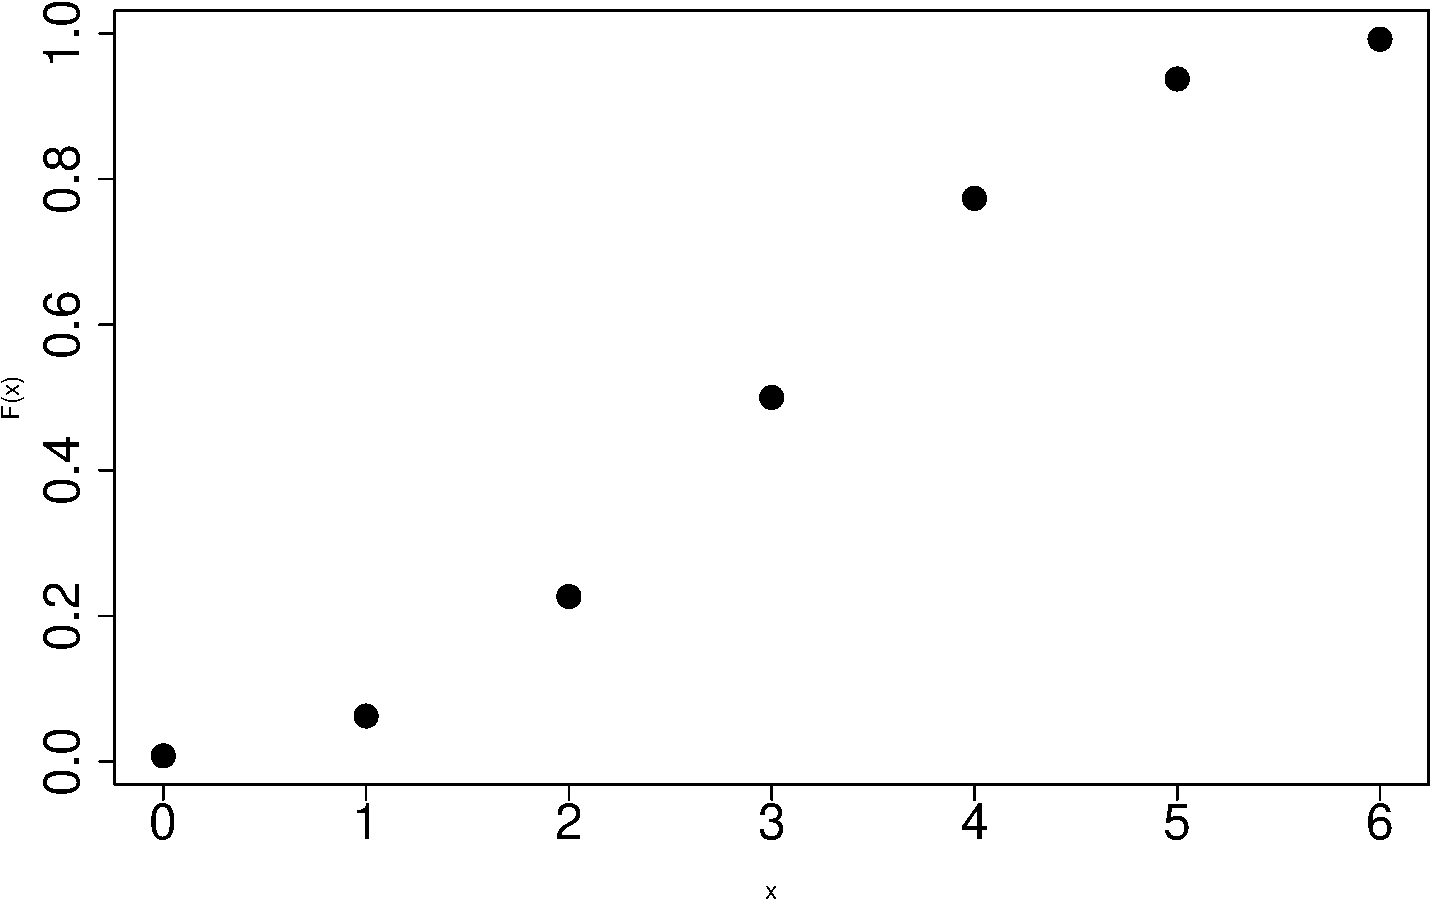
\includegraphics[keepaspectratio]{modulo4_files/figure-beamer/unnamed-chunk-4-2.pdf}}

}

\subcaption{\(\theta = .50\)}

\end{figure}%

\end{minipage}%
%
\begin{minipage}{0.33\linewidth}

\begin{figure}[H]

{\centering \pandocbounded{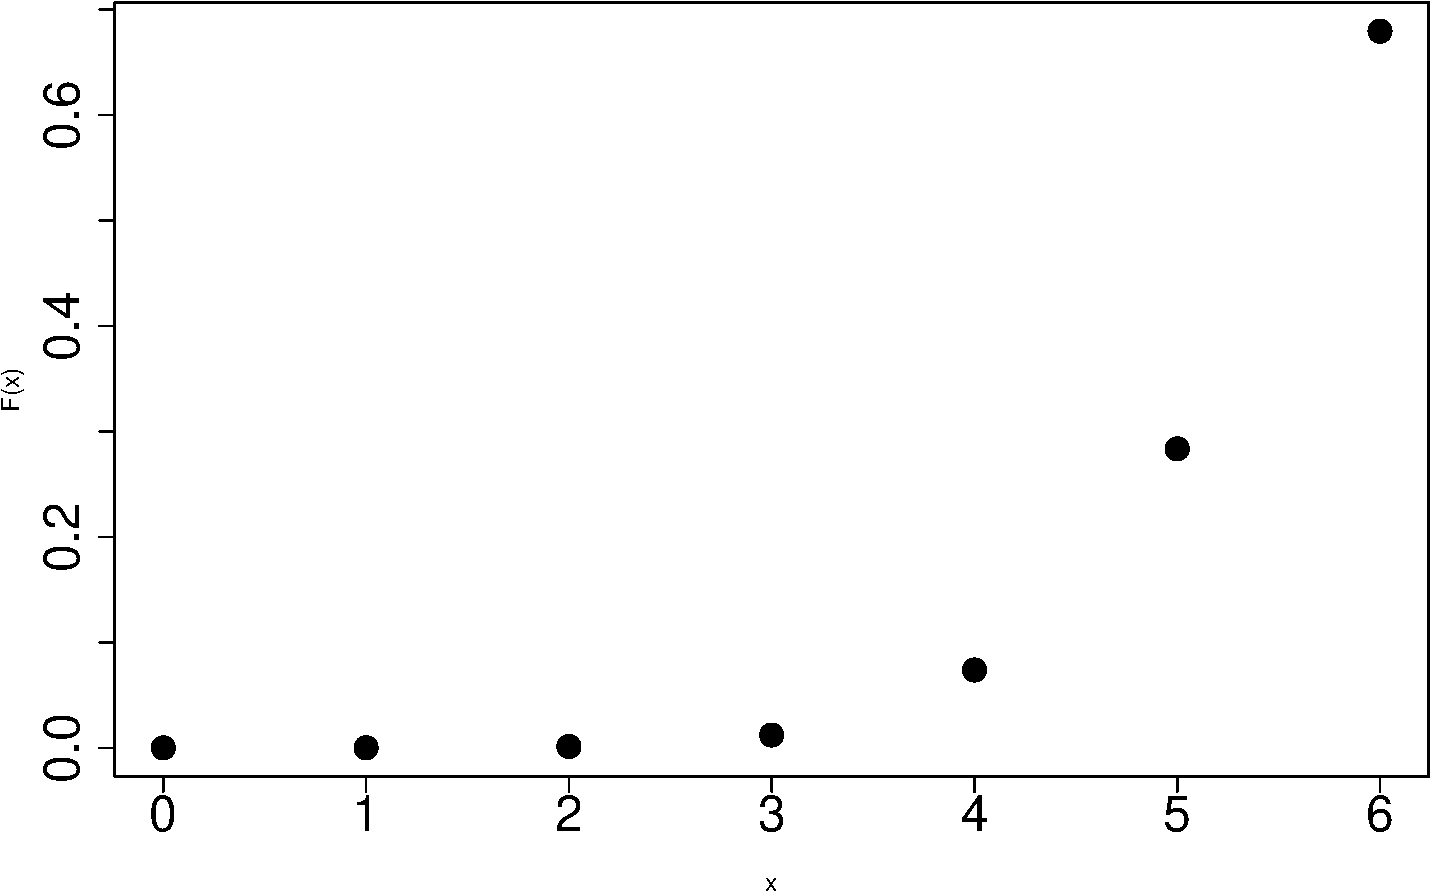
\includegraphics[keepaspectratio]{modulo4_files/figure-beamer/unnamed-chunk-4-3.pdf}}

}

\subcaption{\(\theta = .85\)}

\end{figure}%

\end{minipage}%
\newline
\begin{minipage}{0.33\linewidth}
Probabilità cumulata della binomiale con
\(S = \{0,1, \ldots, 6 \}\)\end{minipage}%

\end{figure}%
\end{frame}

\begin{frame}{}
\phantomsection\label{section-6}
\begin{figure}

\begin{minipage}{0.33\linewidth}

\begin{figure}[H]

{\centering \pandocbounded{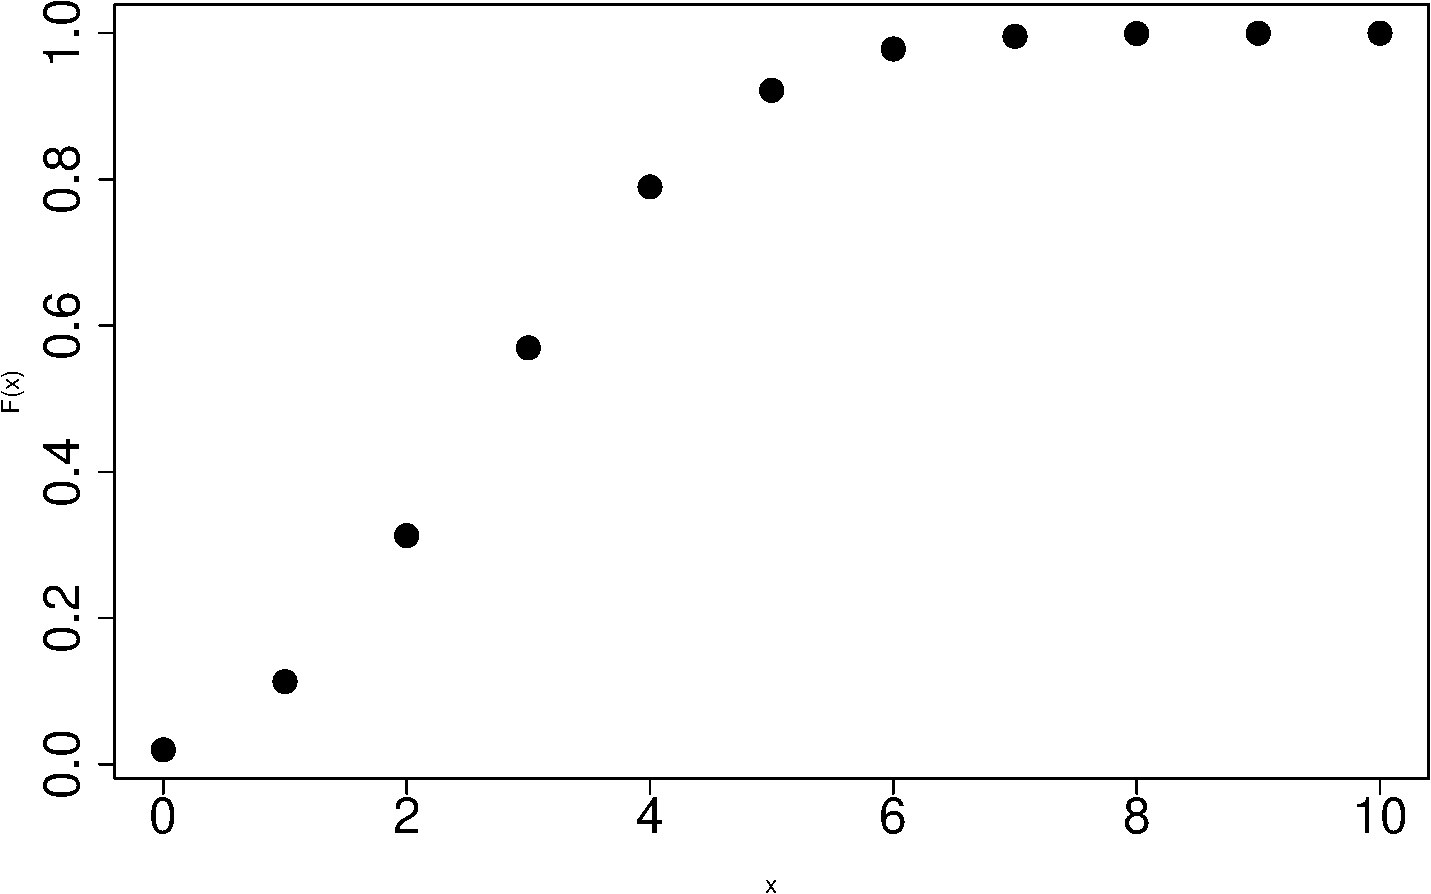
\includegraphics[keepaspectratio]{modulo4_files/figure-beamer/unnamed-chunk-5-1.pdf}}

}

\subcaption{\(\theta = .30\)}

\end{figure}%

\end{minipage}%
%
\begin{minipage}{0.33\linewidth}

\begin{figure}[H]

{\centering \pandocbounded{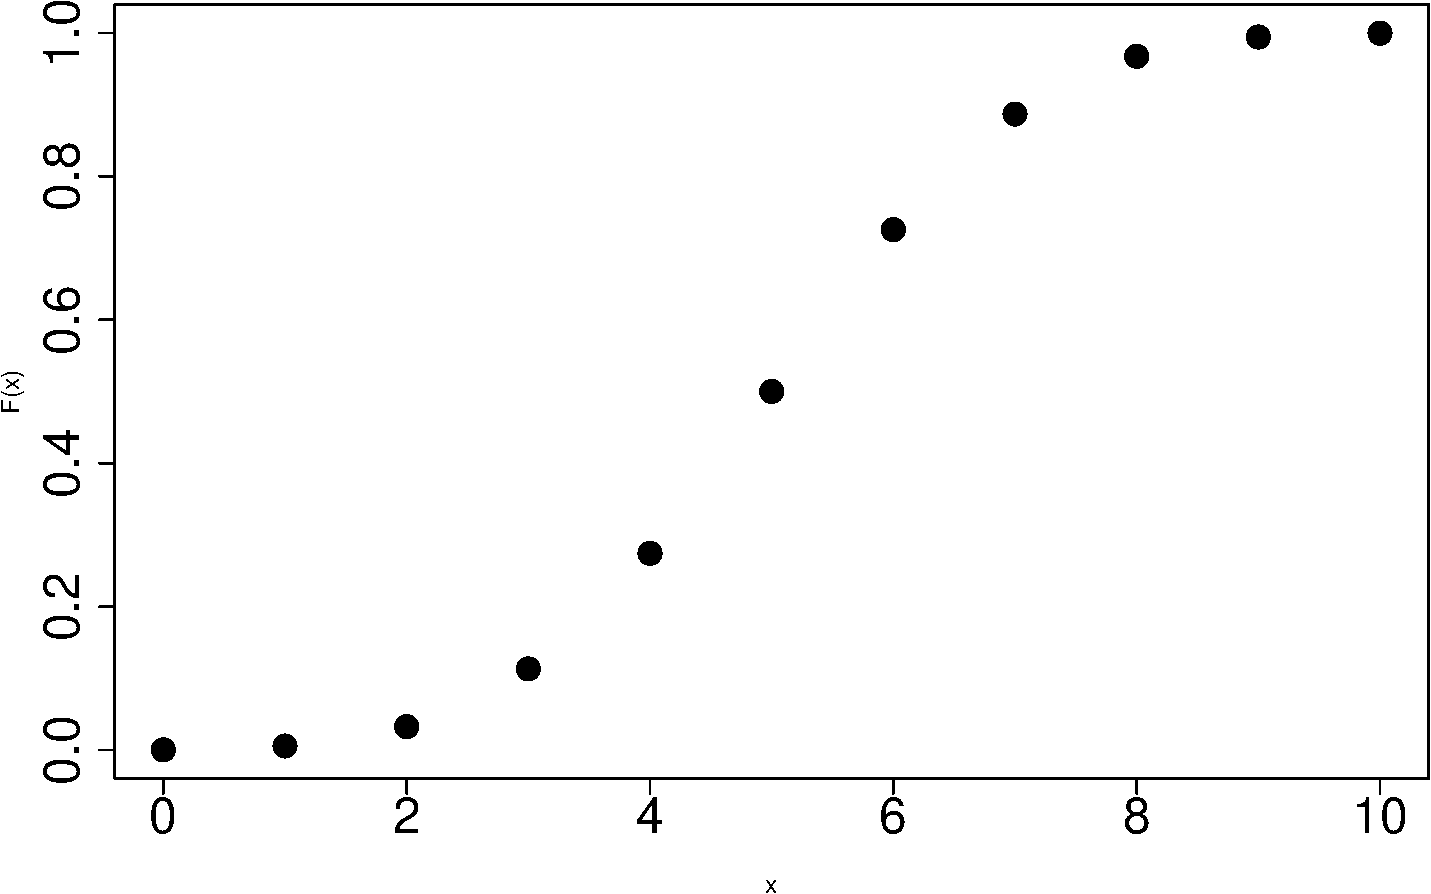
\includegraphics[keepaspectratio]{modulo4_files/figure-beamer/unnamed-chunk-5-2.pdf}}

}

\subcaption{\(\theta = .50\)}

\end{figure}%

\end{minipage}%
%
\begin{minipage}{0.33\linewidth}

\begin{figure}[H]

{\centering \pandocbounded{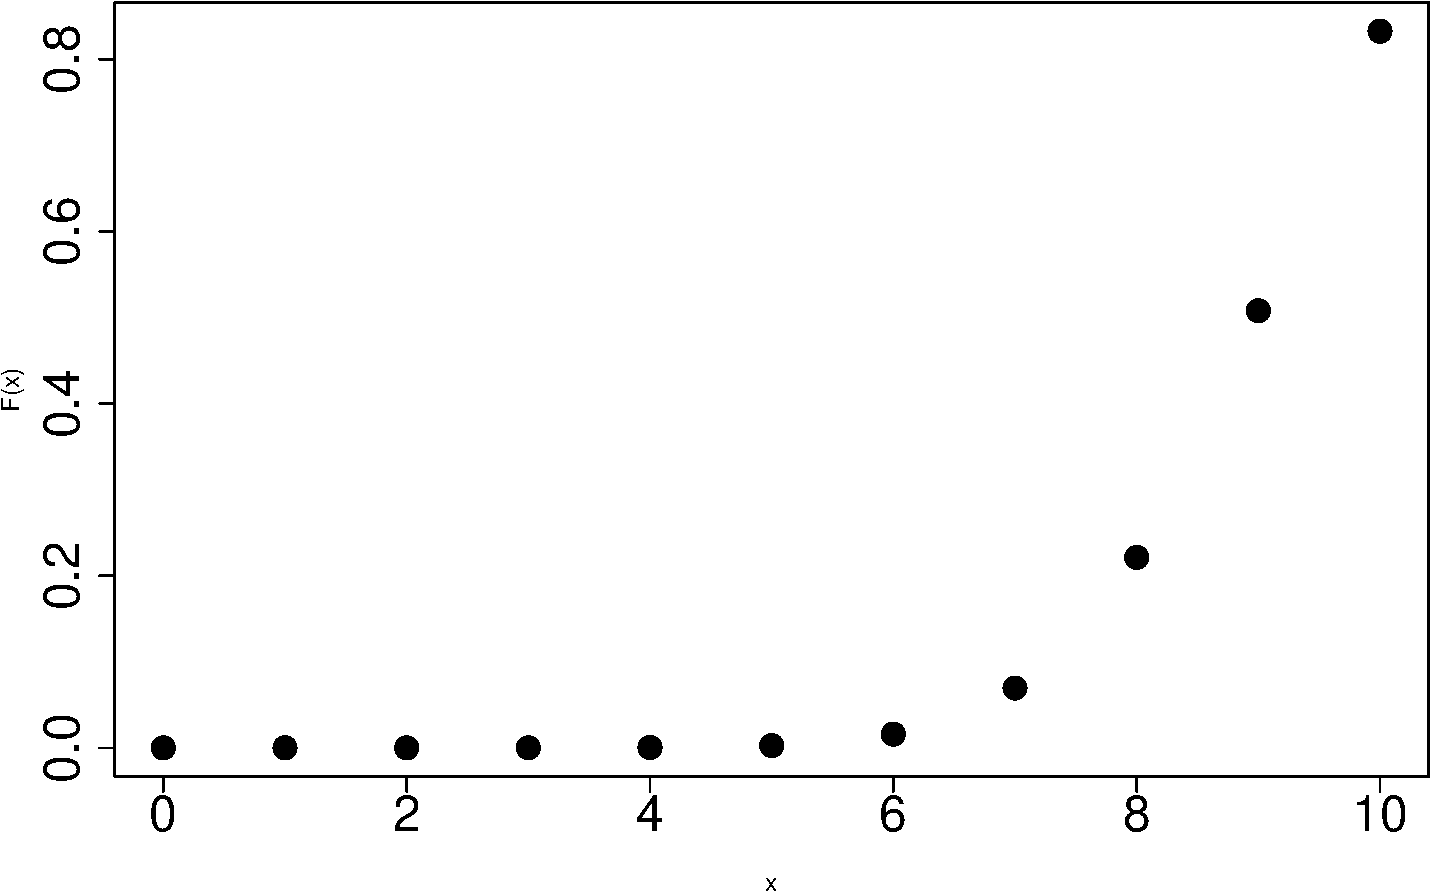
\includegraphics[keepaspectratio]{modulo4_files/figure-beamer/unnamed-chunk-5-3.pdf}}

}

\subcaption{\(\theta = .85\)}

\end{figure}%

\end{minipage}%
\newline
\begin{minipage}{0.33\linewidth}
Probabilità cumulata della binomiale con
\(S = \{0,1, \ldots, 10 \}\)\end{minipage}%

\end{figure}%
\end{frame}

\begin{frame}{}
\phantomsection\label{section-7}
\begin{figure}

\begin{minipage}{0.33\linewidth}

\begin{figure}[H]

{\centering \pandocbounded{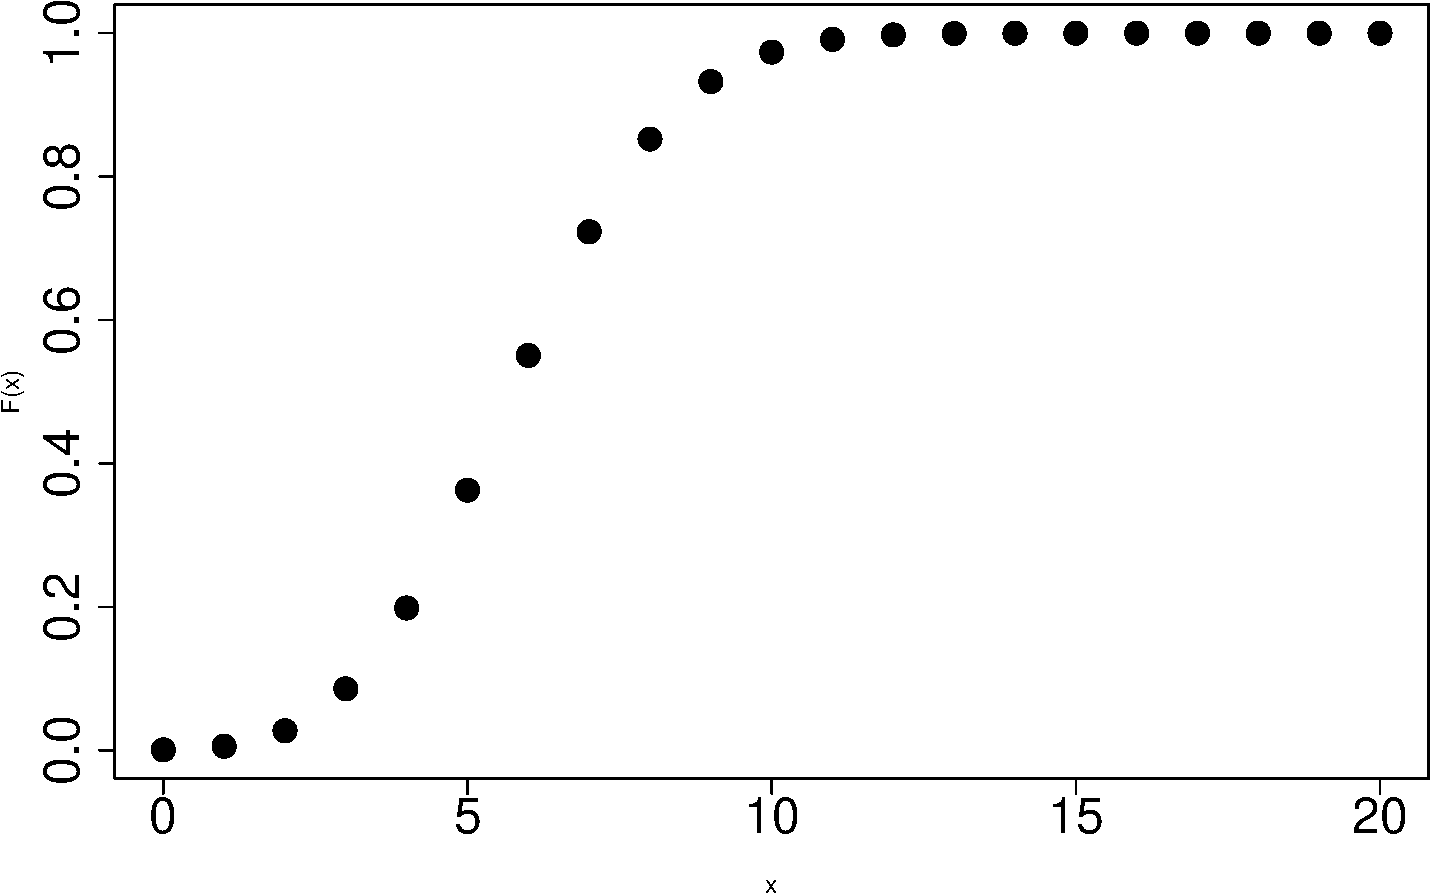
\includegraphics[keepaspectratio]{modulo4_files/figure-beamer/unnamed-chunk-6-1.pdf}}

}

\subcaption{\(\theta = .30\)}

\end{figure}%

\end{minipage}%
%
\begin{minipage}{0.33\linewidth}

\begin{figure}[H]

{\centering \pandocbounded{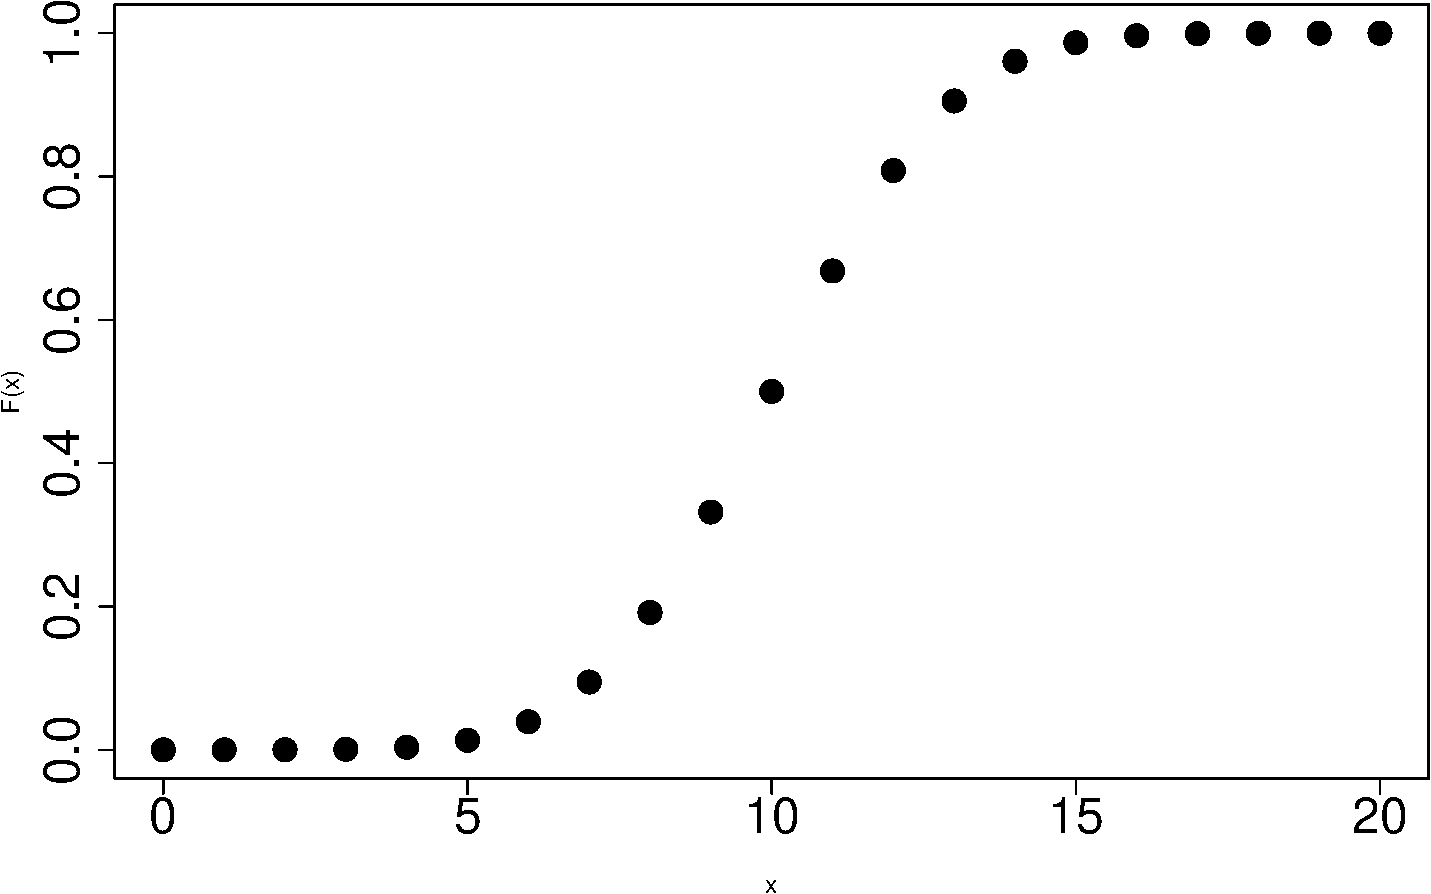
\includegraphics[keepaspectratio]{modulo4_files/figure-beamer/unnamed-chunk-6-2.pdf}}

}

\subcaption{\(\theta = .50\)}

\end{figure}%

\end{minipage}%
%
\begin{minipage}{0.33\linewidth}

\begin{figure}[H]

{\centering \pandocbounded{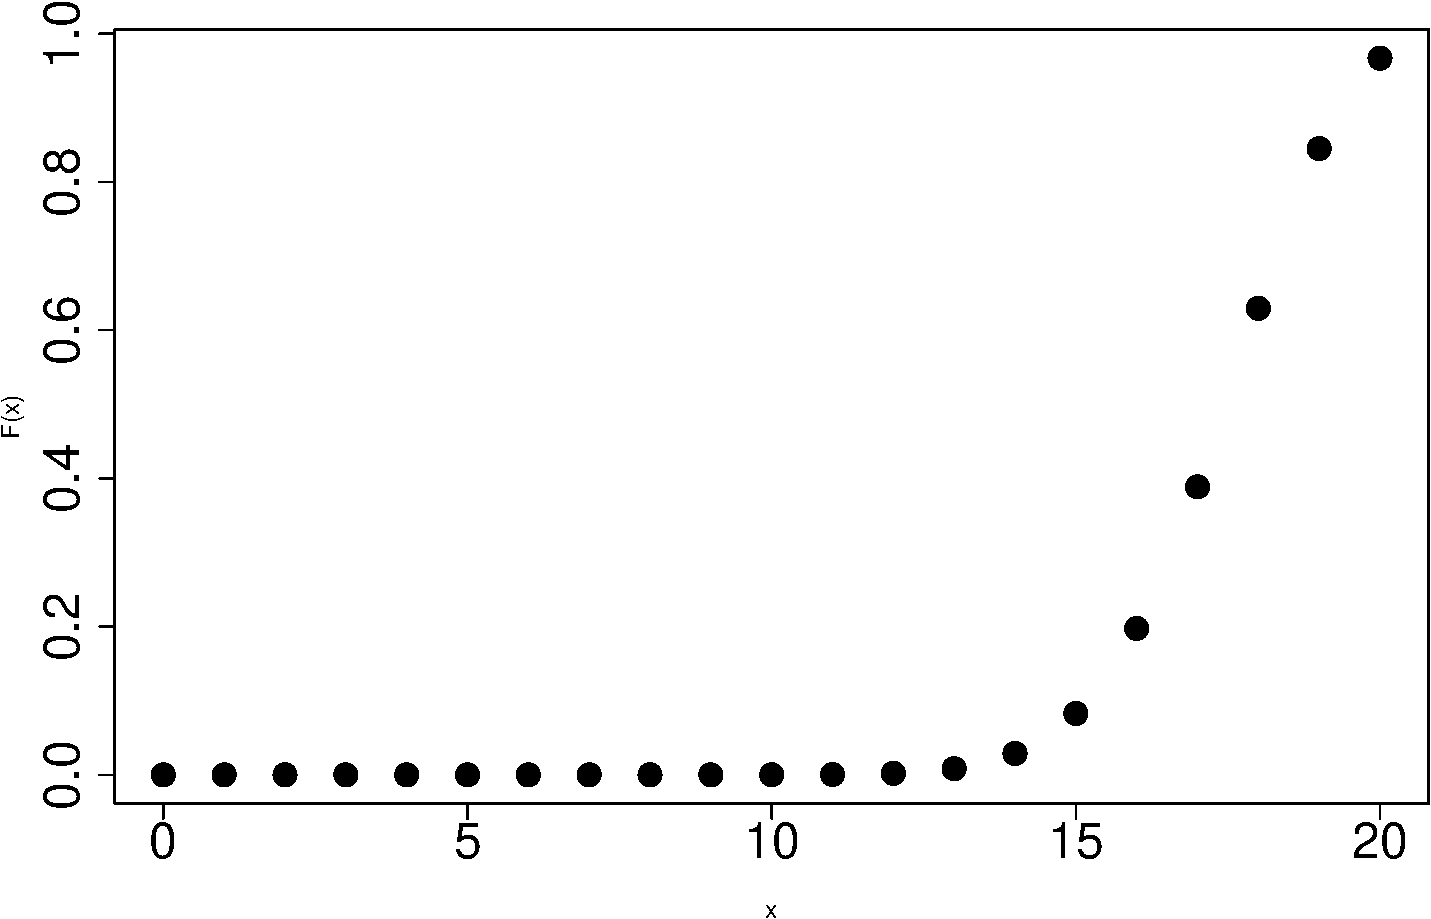
\includegraphics[keepaspectratio]{modulo4_files/figure-beamer/unnamed-chunk-6-3.pdf}}

}

\subcaption{\(\theta = .85\)}

\end{figure}%

\end{minipage}%
\newline
\begin{minipage}{0.33\linewidth}
Probabilità cumulata della binomiale con
\(S = \{0,1, \ldots, 20 \}\)\end{minipage}%

\end{figure}%
\end{frame}

\begin{frame}[fragile]{}
\phantomsection\label{section-8}
\begin{longtable}[]{@{}
  >{\raggedright\arraybackslash}p{(\linewidth - 2\tabcolsep) * \real{0.4348}}
  >{\raggedright\arraybackslash}p{(\linewidth - 2\tabcolsep) * \real{0.5652}}@{}}
\toprule\noalign{}
\begin{minipage}[b]{\linewidth}\raggedright
Funzione
\end{minipage} & \begin{minipage}[b]{\linewidth}\raggedright
Descrizione
\end{minipage} \\
\midrule\noalign{}
\endhead
\texttt{dbinom(x,\ size,\ prob)} & Restituisce i \emph{valori di massa}
associati al vettore discreto \texttt{x} di una distribuzione binomiale
con \texttt{n} esperimenti bernoulliani e probabilità \texttt{prob} per
l'evento target. Con \texttt{lower.tail=FALSE} calcola la probabilità
complementare. \\
\texttt{pbinom(x,\ size,\ prob)} & Restituisce i \emph{valori di
probabilità cumulata} associati al vettore discreto \texttt{x}. \\
\texttt{qbinom(p,\ size,\ prob)} & Restituisce i \emph{valori dei
quantili} associati al vettore di probabilità \texttt{p}. \\
\texttt{rbinom(n,\ size,\ prob)} & Restituisce un vettore casuale di
\texttt{n} osservazioni indipendenti campionate da una distribuzione
binomiale. \\
\bottomrule\noalign{}
\end{longtable}
\end{frame}

\section{Funzioni di probabilità
Continue}\label{funzioni-di-probabilituxe0-continue}

\subsection{Definizioni generali}\label{definizioni-generali-1}

\begin{frame}{}
\phantomsection\label{section-9}
Sia \(X\) una variabile casuale continua distribuita secondo la funzione
di densità \(f_X(x|\theta)\):

\[f_X : \mathbb{R} \times \Theta \to \mathbb{R}^+\]

\(f_X\) è una funzione di densità parametrica con parametri
\(\theta \in \Theta\).

La \emph{funzione di densità cumulata} \(F_X(x|\theta)\) è definita come

\[F_X(x|\theta) = \Pr[X \leq x]
= \int_{-\infty}^x f_X(z|\theta)\,dz\]

dove chiaramente

\[F_X : \mathbb{R} \times \Theta \to [0,1]\]
\end{frame}

\begin{frame}{}
\phantomsection\label{section-10}
Infine, la \emph{funzione quantile+} \(q_X(p|\theta)\) è definita come
la funzione inversa di \(F_X\):

\[q_X(p|\theta) = F_X^{-1}(p|\theta)
= x \in \mathbb{R} \ \ \text{tale che} \ \ p = F_X(x|\theta)\]

dove

\[q_X : [0,1] \times \Theta \to \mathbb{R}\]

Nota che in generale

\[q_X(p|\theta) = F_X^{-1}(p|\theta) 
\quad \text{sse} \quad 
F_X(x|\theta) = q_X^{-1}(x|\theta).\]
\end{frame}

\subsection{Normale}\label{normale}

\begin{frame}{}
\phantomsection\label{section-11}
\begin{columns}[T]
\begin{column}{0.5\linewidth}
Distribuzione Normale

\[f(x) = {\displaystyle {\dfrac {1}{\sigma {\sqrt {2\pi }}}}e^{-{\dfrac {1}{2}}\left({\dfrac {x-\mu }{\sigma }}\right)^{2}}}\]

\(\theta = (\mu, \sigma^2)\),
\(\Theta = (\mathbb{R} \times \mathbb{R}^+)\)
\end{column}

\begin{column}{0.5\linewidth}
Distribuzione Normale Standard

\[f(z) = \dfrac{1}{\sqrt{2\pi}} e^{-\dfrac{1}{2}z^2}\]

\(\theta = z\), \(\Theta = (\mathbb{R})\)
\end{column}
\end{columns}
\end{frame}

\begin{frame}{}
\phantomsection\label{section-12}
\small

\textbf{VALORI}:

\begin{quote}
vanno da \(-\infty\) a \(+ \infty\) (in ascissa si trovano tutti i
valori di \(x\); in ordinata le frequenze \(f(x)\) di ciascun valore)
\end{quote}

\textbf{SIMMETRICA}

\begin{quote}
rispetto alla \(Y\) massima (\(f(x)=\) punto più alto
\(\Rightarrow x = \mu\)) (solo un valore centrale ha la frequenza
massima; i valori più bassi e più alti compaiono rispettivamente con
frequenza crescente e decrescente)
\end{quote}

\textbf{UNIMODALE}

\(\mu = Mo=Me\)

\textbf{ASINTOTICA}:

\begin{quote}
si avvicina all'asse delle \(X\) senza mai toccarlo. La curva mostra due
\textbf{PUNTI DI FLESSO}: da concava diventa convessa nella metà
sinistra e da convessa diventa concava nella metà destra (in
corrispondenza di valori di x uguali alla media meno o più una ds)
\end{quote}
\end{frame}

\begin{frame}{}
\phantomsection\label{section-13}
L'area sottesa alla curva normale rappresenta la PROBABILITA' degli
intervalli

\[\int_{-\infty}^{+\infty} f(x) dX =1\]

\begin{center}
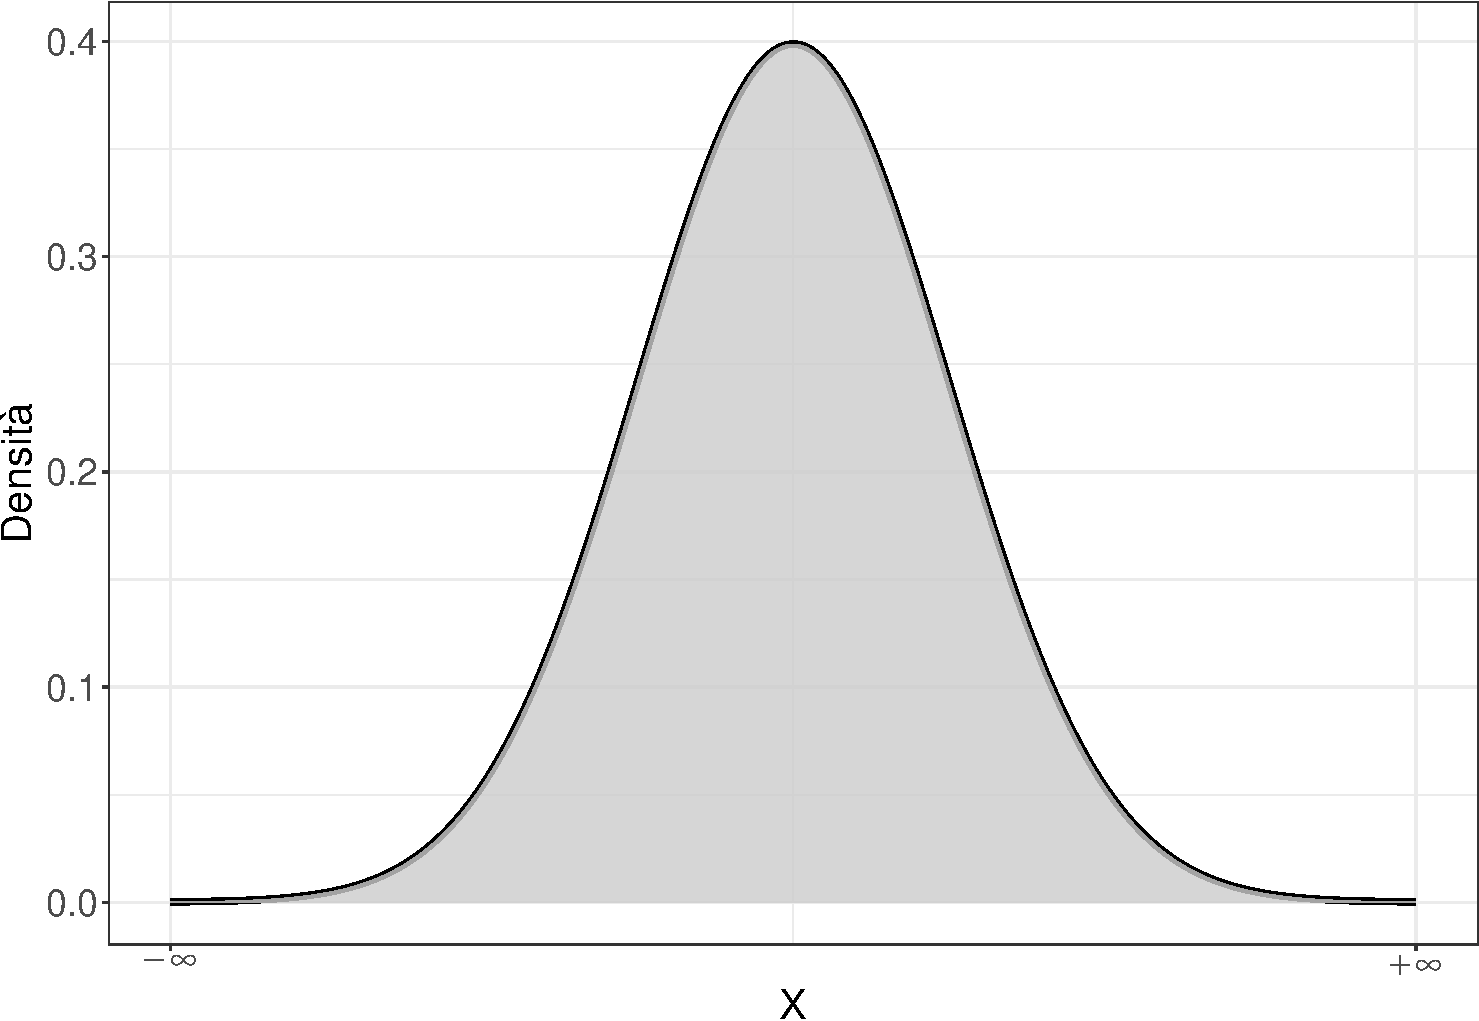
\includegraphics[width=0.5\linewidth,height=\textheight,keepaspectratio]{modulo4_files/figure-beamer/unnamed-chunk-7-1.pdf}
\end{center}
\end{frame}

\begin{frame}[plain]{}
\phantomsection\label{section-14}
\begin{figure}

\begin{minipage}{0.50\linewidth}
\pandocbounded{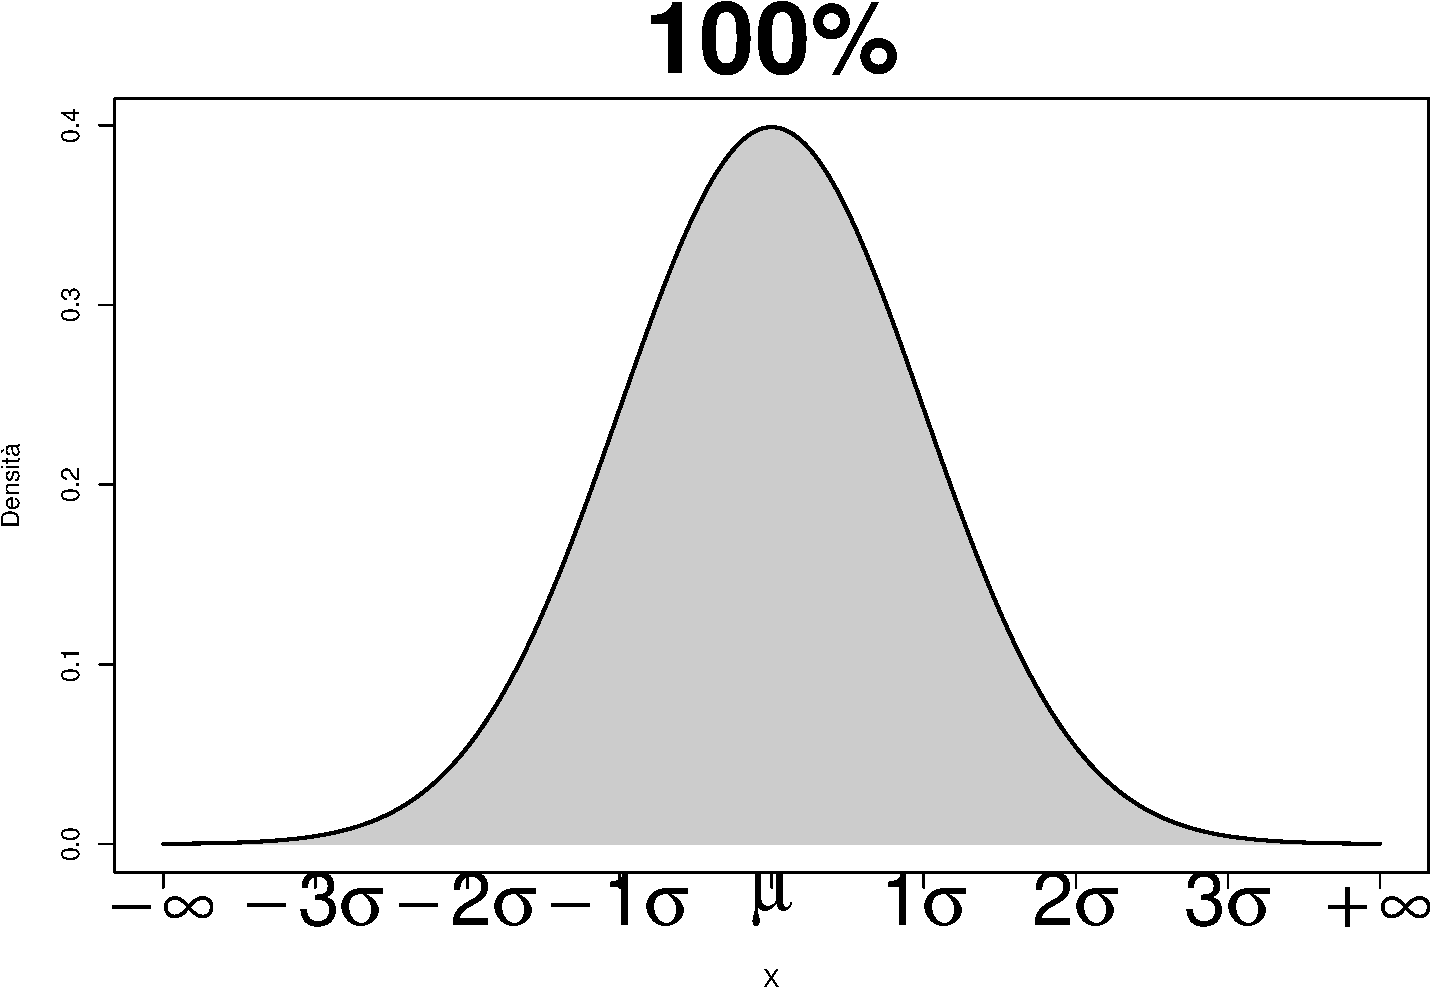
\includegraphics[keepaspectratio]{modulo4_files/figure-beamer/unnamed-chunk-8-1.pdf}}\end{minipage}%
%
\begin{minipage}{0.50\linewidth}
\pandocbounded{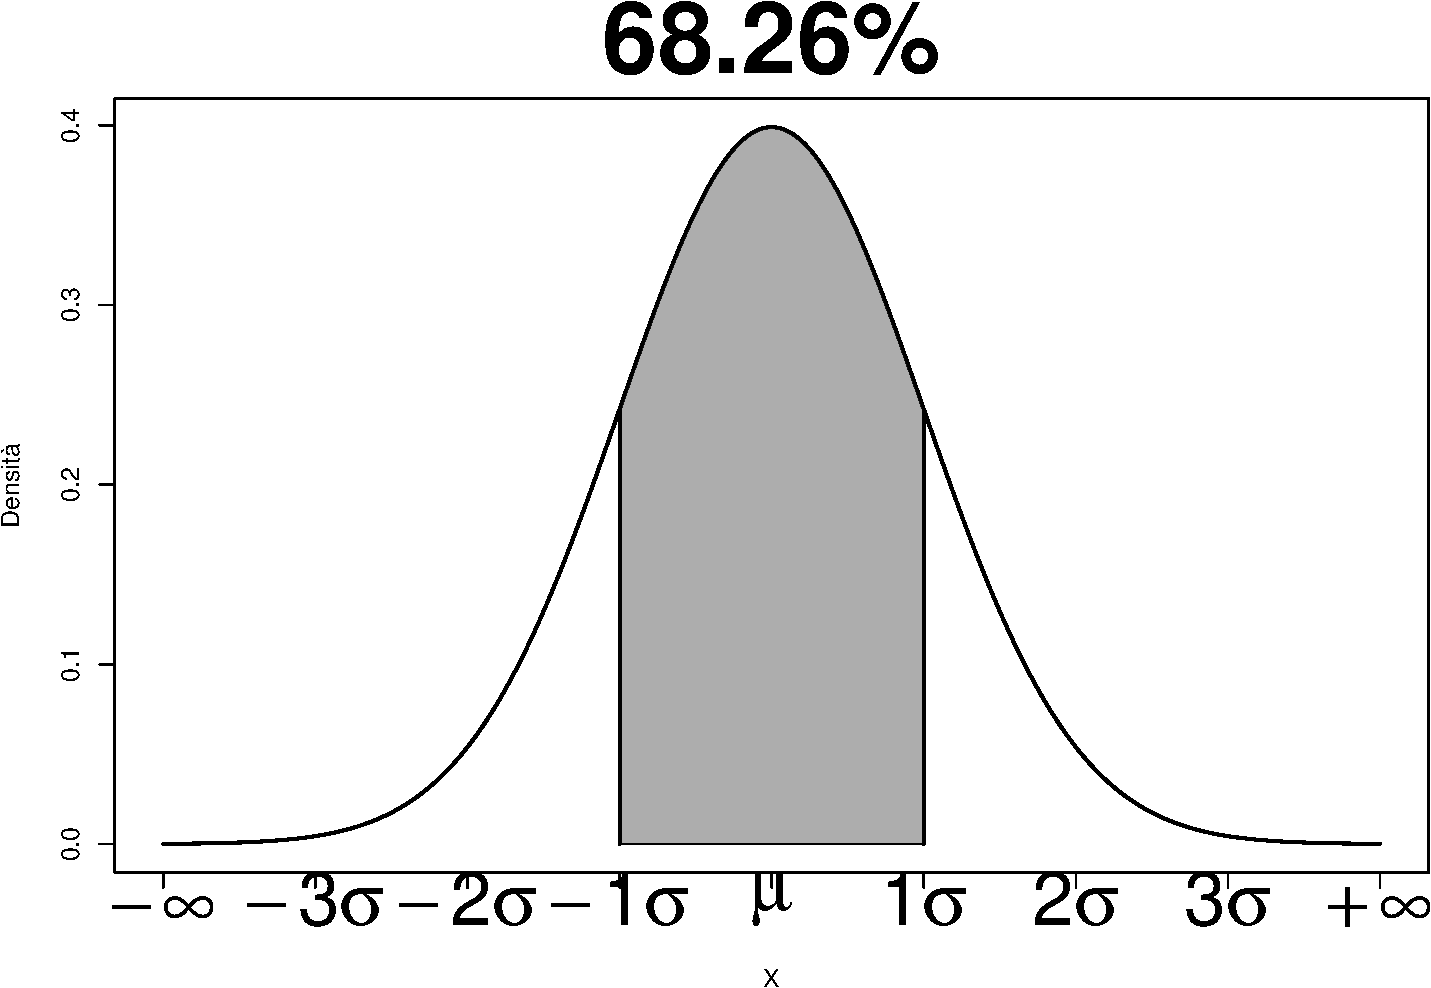
\includegraphics[keepaspectratio]{modulo4_files/figure-beamer/unnamed-chunk-8-2.pdf}}\end{minipage}%
\newline
\begin{minipage}{0.50\linewidth}
\pandocbounded{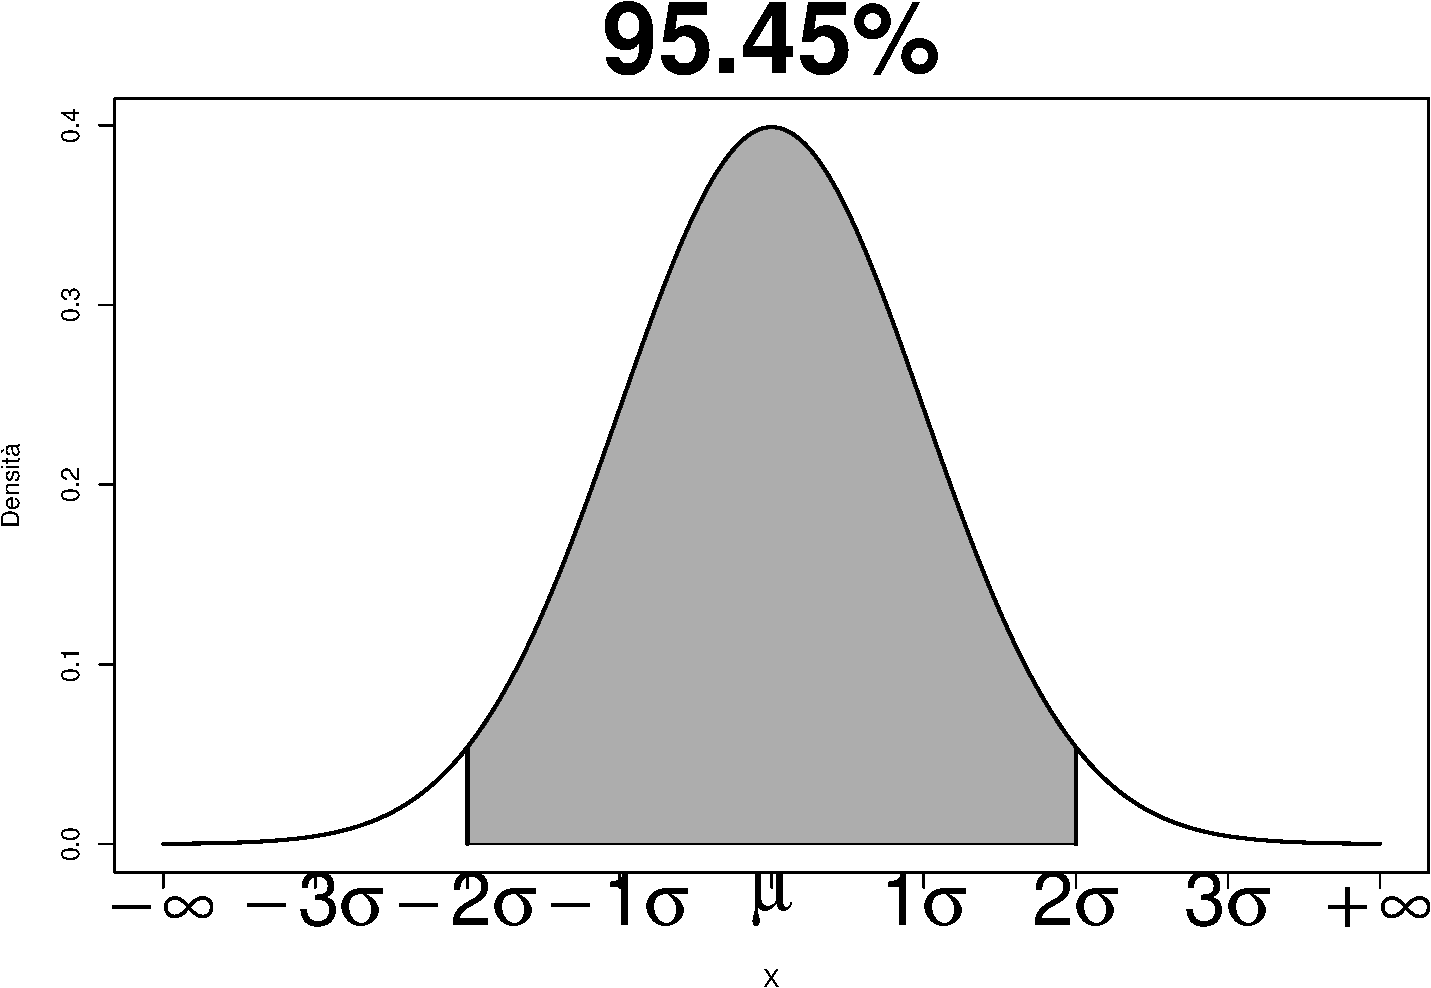
\includegraphics[keepaspectratio]{modulo4_files/figure-beamer/unnamed-chunk-8-3.pdf}}\end{minipage}%
%
\begin{minipage}{0.50\linewidth}
\pandocbounded{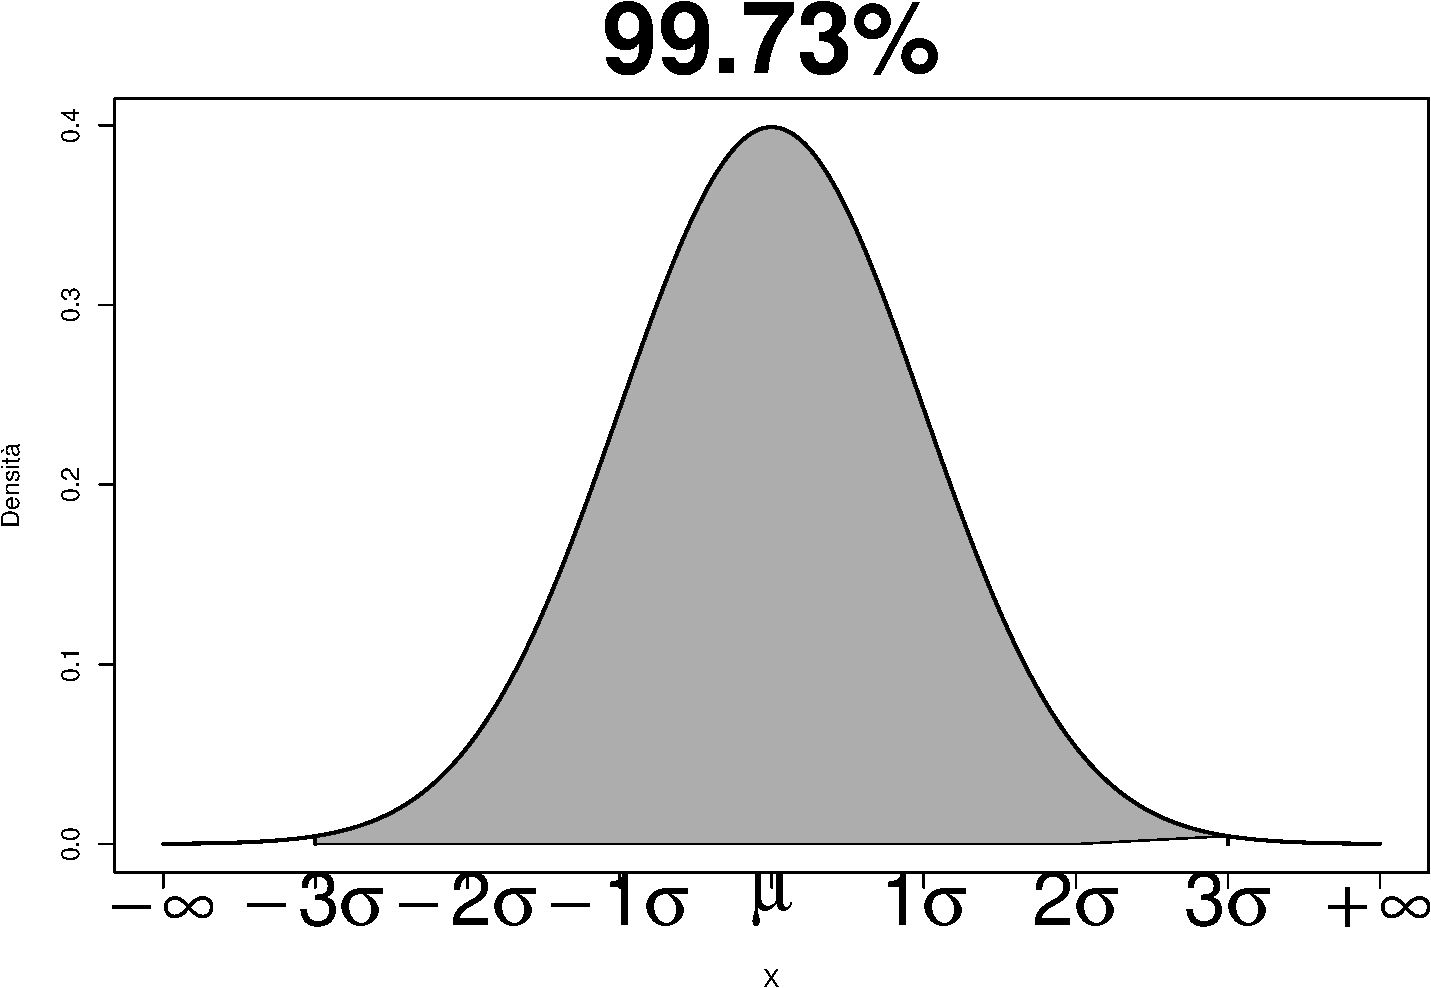
\includegraphics[keepaspectratio]{modulo4_files/figure-beamer/unnamed-chunk-8-4.pdf}}\end{minipage}%

\end{figure}%
\end{frame}

\begin{frame}{}
\phantomsection\label{section-15}
\begin{figure}

\begin{minipage}{0.33\linewidth}

\begin{figure}[H]

{\centering \pandocbounded{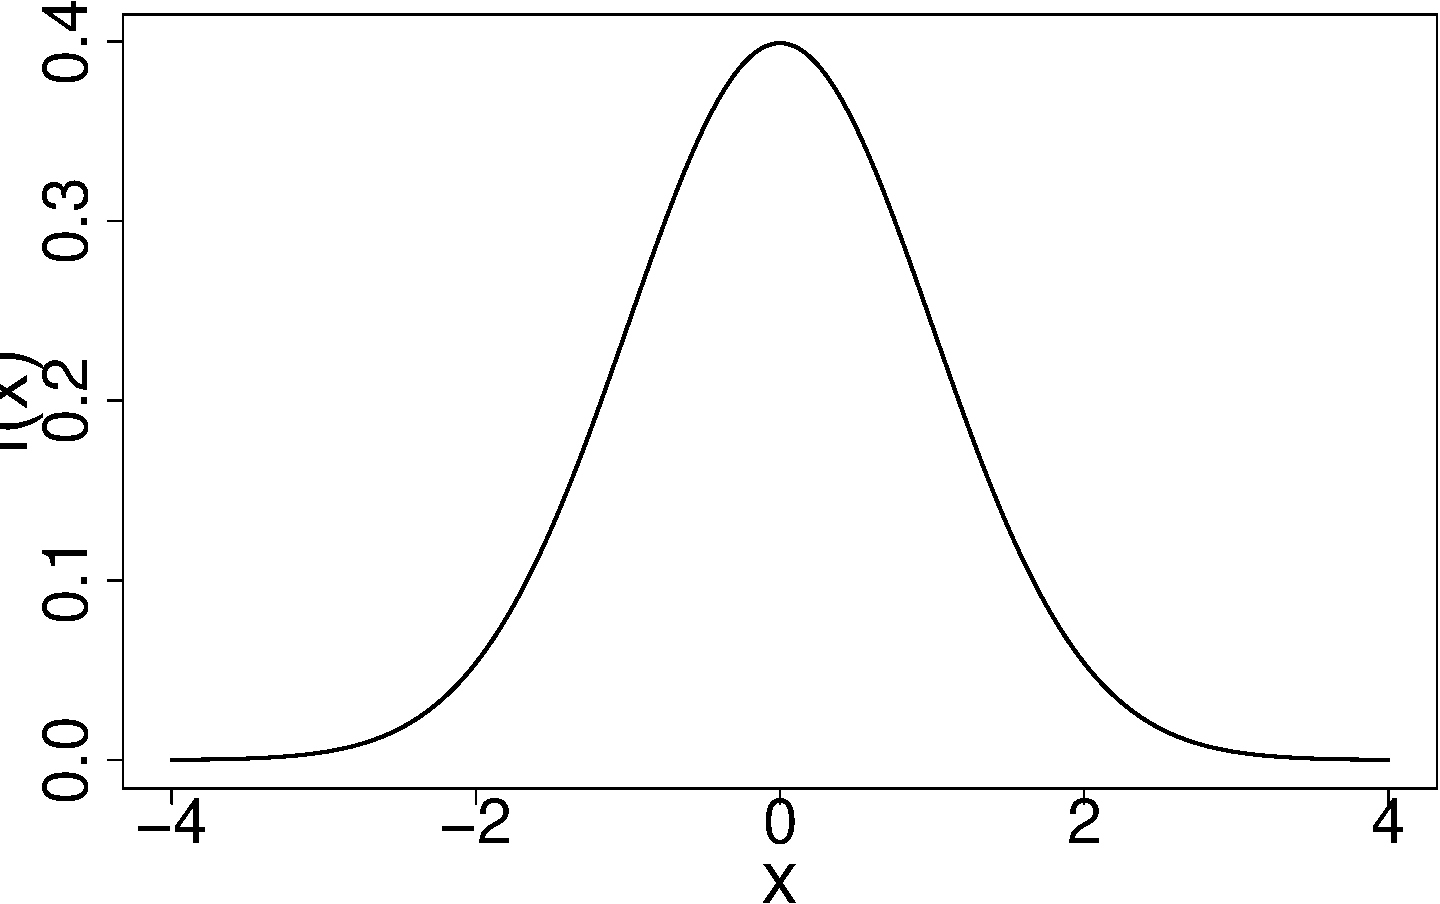
\includegraphics[keepaspectratio]{modulo4_files/figure-beamer/unnamed-chunk-9-1.pdf}}

}

\subcaption{Densità}

\end{figure}%

\end{minipage}%
%
\begin{minipage}{0.33\linewidth}

\begin{figure}[H]

{\centering \pandocbounded{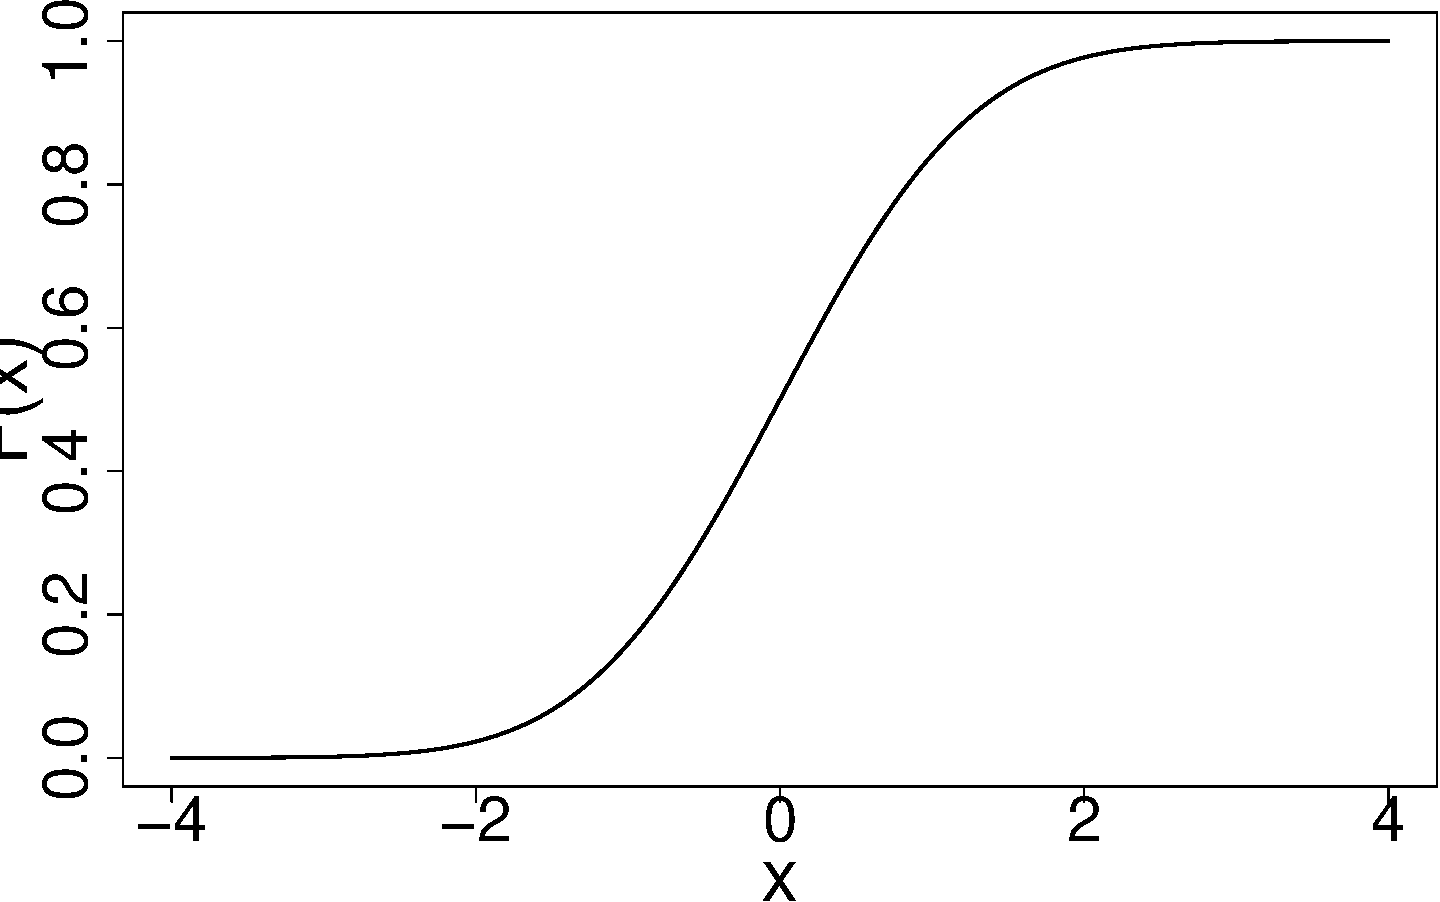
\includegraphics[keepaspectratio]{modulo4_files/figure-beamer/unnamed-chunk-9-2.pdf}}

}

\subcaption{Cumulata}

\end{figure}%

\end{minipage}%
%
\begin{minipage}{0.33\linewidth}

\begin{figure}[H]

{\centering \pandocbounded{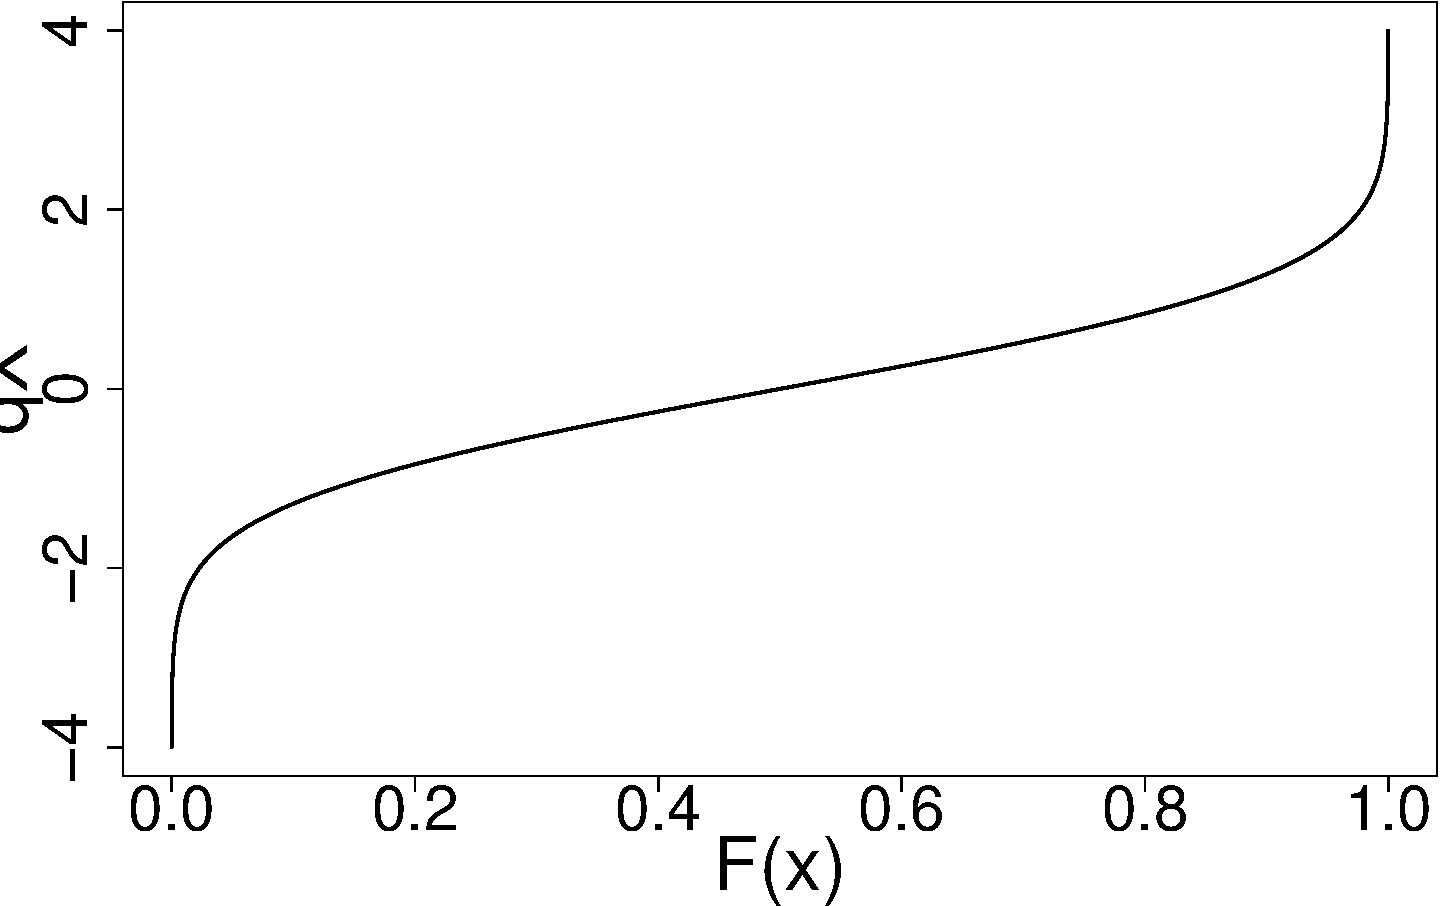
\includegraphics[keepaspectratio]{modulo4_files/figure-beamer/unnamed-chunk-9-3.pdf}}

}

\subcaption{Quantile}

\end{figure}%

\end{minipage}%
\newline
\begin{minipage}{0.33\linewidth}
Distribuzione normale\end{minipage}%

\end{figure}%
\end{frame}

\begin{frame}[fragile]{}
\phantomsection\label{section-16}
\begin{longtable}[]{@{}
  >{\raggedright\arraybackslash}p{(\linewidth - 2\tabcolsep) * \real{0.4348}}
  >{\raggedright\arraybackslash}p{(\linewidth - 2\tabcolsep) * \real{0.5652}}@{}}
\toprule\noalign{}
\begin{minipage}[b]{\linewidth}\raggedright
Funzione
\end{minipage} & \begin{minipage}[b]{\linewidth}\raggedright
Descrizione
\end{minipage} \\
\midrule\noalign{}
\endhead
\texttt{dnorm(x,\ mean,\ sd)} & Restituisce i \emph{valori di densità
associati} al valore quantitativo \texttt{x} di una distribuzione
normale con media e deviazione standard. \\
\texttt{pnorm(x,\ mean,\ sd)} & Restituisce i \emph{valori di
probabilità cumulata} associati al vettore \texttt{x}. \\
\texttt{qnorm(p,\ mean,\ sd)} & Restituisce i \emph{valori dei quantili}
associati al vettore di probabilità \texttt{p} di una distribuzione
normale (\texttt{0\ \textless{}=\ p\ \textless{}=\ 1}). \\
\texttt{rnorm(n,\ mean,\ sd)} & Genera un vettore casuale di \texttt{n}
osservazioni indipendenti campionate da una nomrale con media e
deviazione standard. \\
\bottomrule\noalign{}
\end{longtable}
\end{frame}

\begin{frame}{}
\phantomsection\label{section-17}
\(\theta = (\mu, \sigma^2)\),
\(\Theta = (\mathbb{R} \times \mathbb{R}^+)\)

\begin{columns}[T]
\begin{column}{0.8\linewidth}
\pandocbounded{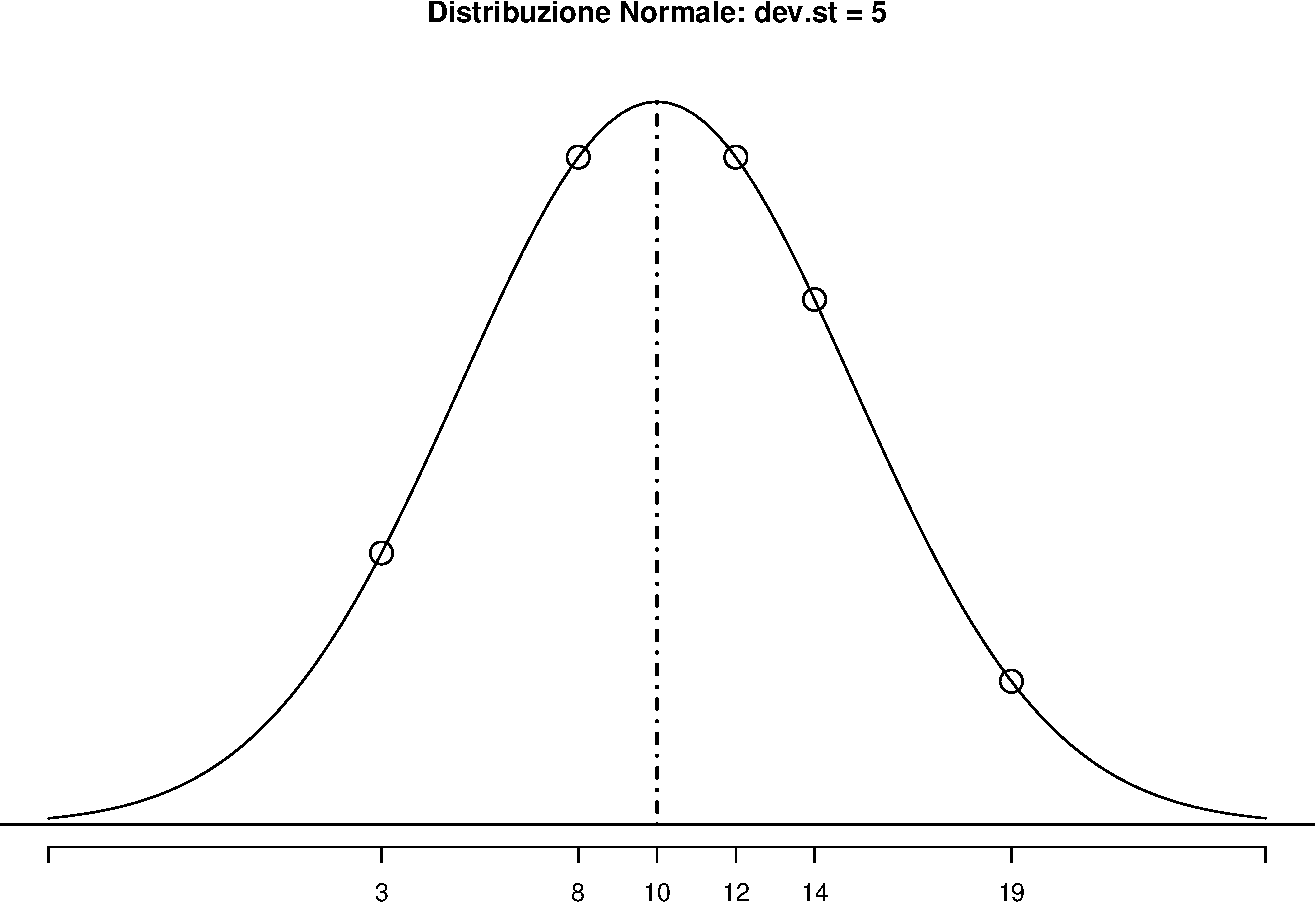
\includegraphics[keepaspectratio]{modulo4_files/figure-beamer/unnamed-chunk-10-1.pdf}}
\end{column}

\begin{column}{0.2\linewidth}
\small

\(f(3) = 0.0299\)

\(f(8) = 0.0737\)

\(f(12) = 0.0737\)

\(f(14) = 0.0579\)

\(f(19) = 0.0158\)
\end{column}
\end{columns}
\end{frame}

\begin{frame}{}
\phantomsection\label{section-18}
\begin{columns}[T]
\begin{column}{0.75\linewidth}
\pandocbounded{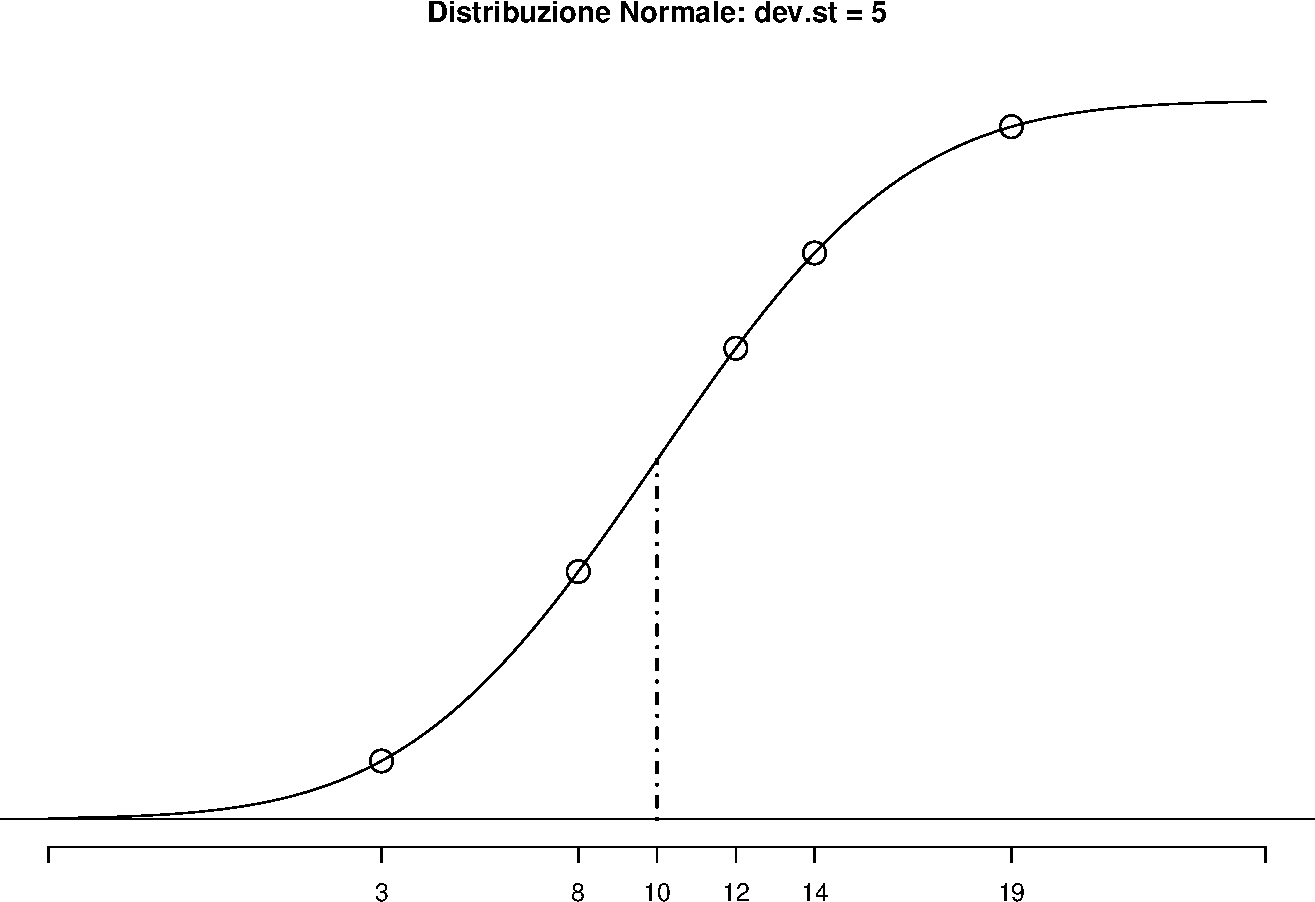
\includegraphics[keepaspectratio]{modulo4_files/figure-beamer/unnamed-chunk-11-1.pdf}}
\end{column}

\begin{column}{0.25\linewidth}
\small

\(F(3) = 0.0808\)

\(F(8) = 0.3446\)

\(F(12) = 0.6554\)

\(F(14) = 0.7881\)

\(F(19) = 0.9641\)

\vspace{5mm}

\(q(0.0808) = 3\)

\(q(0.3446) = 8\)

\(q(0.6554) = 12\)

\(q(0.7881) = 14\)

\(q(0.9641) = 19\)
\end{column}
\end{columns}
\end{frame}

\begin{frame}{}
\phantomsection\label{section-19}
\begin{figure}

\begin{minipage}{0.50\linewidth}

\begin{figure}[H]

{\centering \pandocbounded{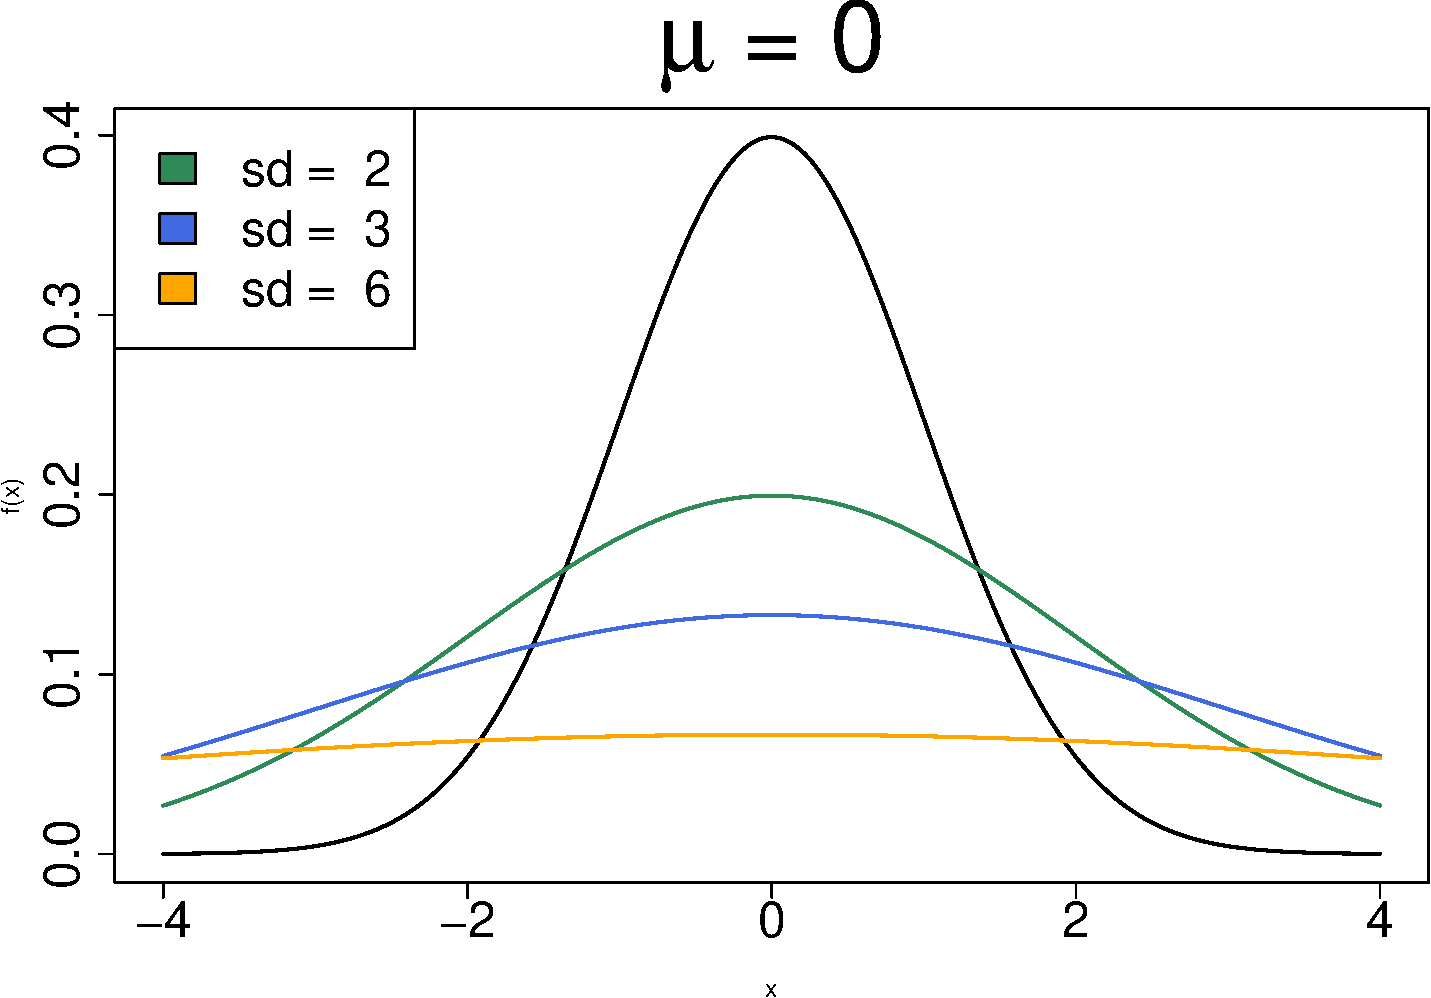
\includegraphics[keepaspectratio]{modulo4_files/figure-beamer/unnamed-chunk-12-1.pdf}}

}

\subcaption{Densità}

\end{figure}%

\end{minipage}%
%
\begin{minipage}{0.50\linewidth}

\begin{figure}[H]

{\centering \pandocbounded{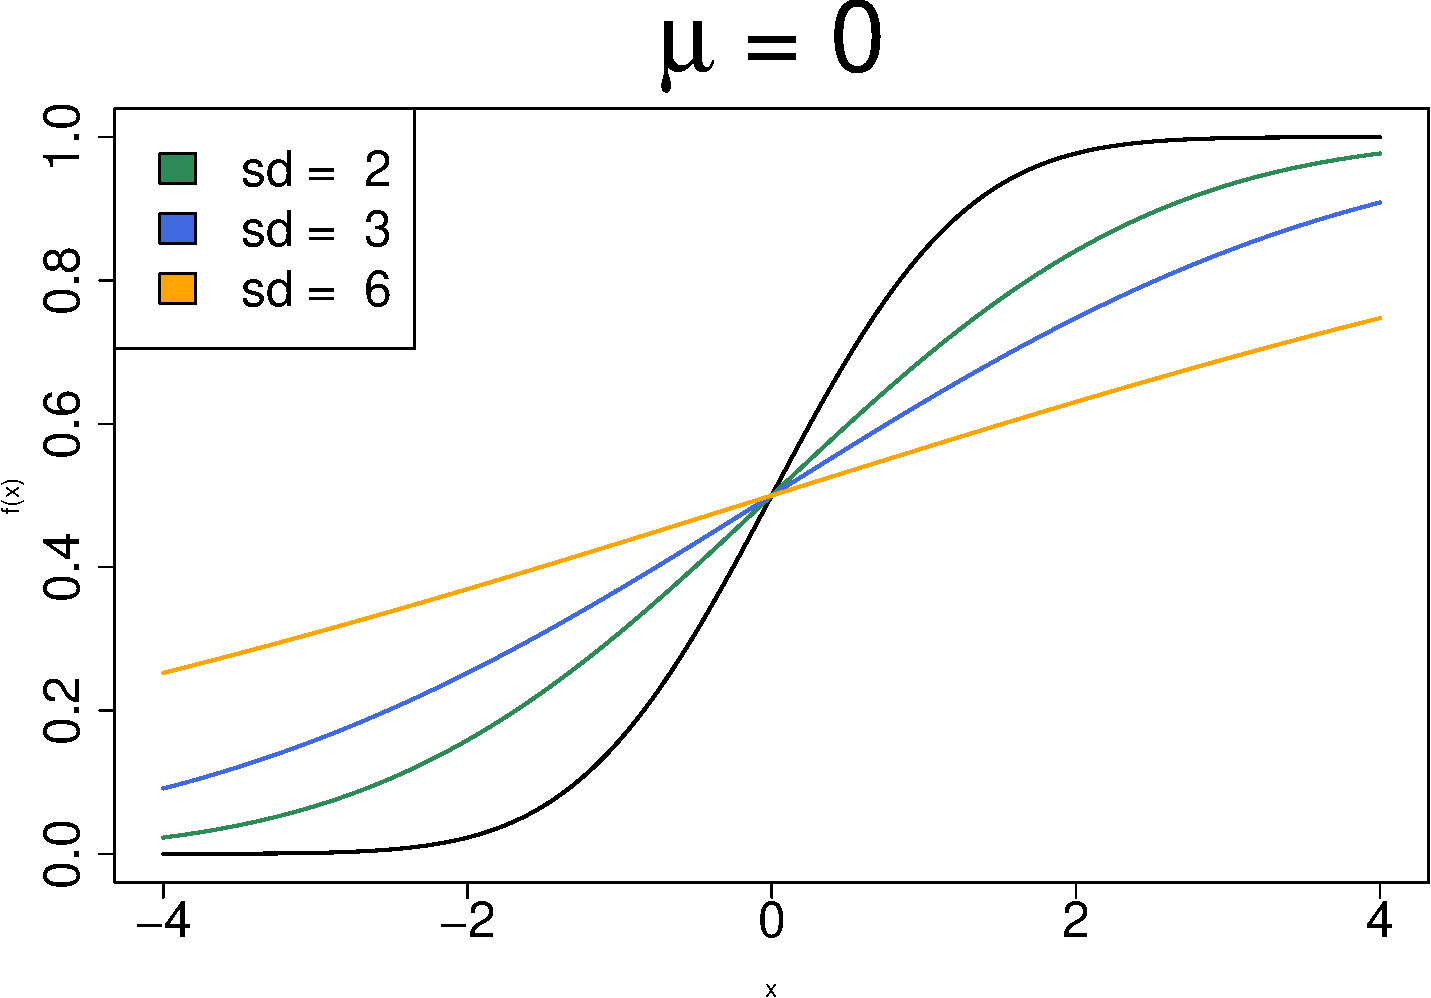
\includegraphics[keepaspectratio]{modulo4_files/figure-beamer/unnamed-chunk-12-2.pdf}}

}

\subcaption{Cumulata}

\end{figure}%

\end{minipage}%
\newline
\begin{minipage}{0.50\linewidth}
Stessa media, diversa SD\end{minipage}%

\end{figure}%
\end{frame}

\begin{frame}{}
\phantomsection\label{section-20}
\begin{figure}

\begin{minipage}{0.50\linewidth}

\begin{figure}[H]

{\centering \pandocbounded{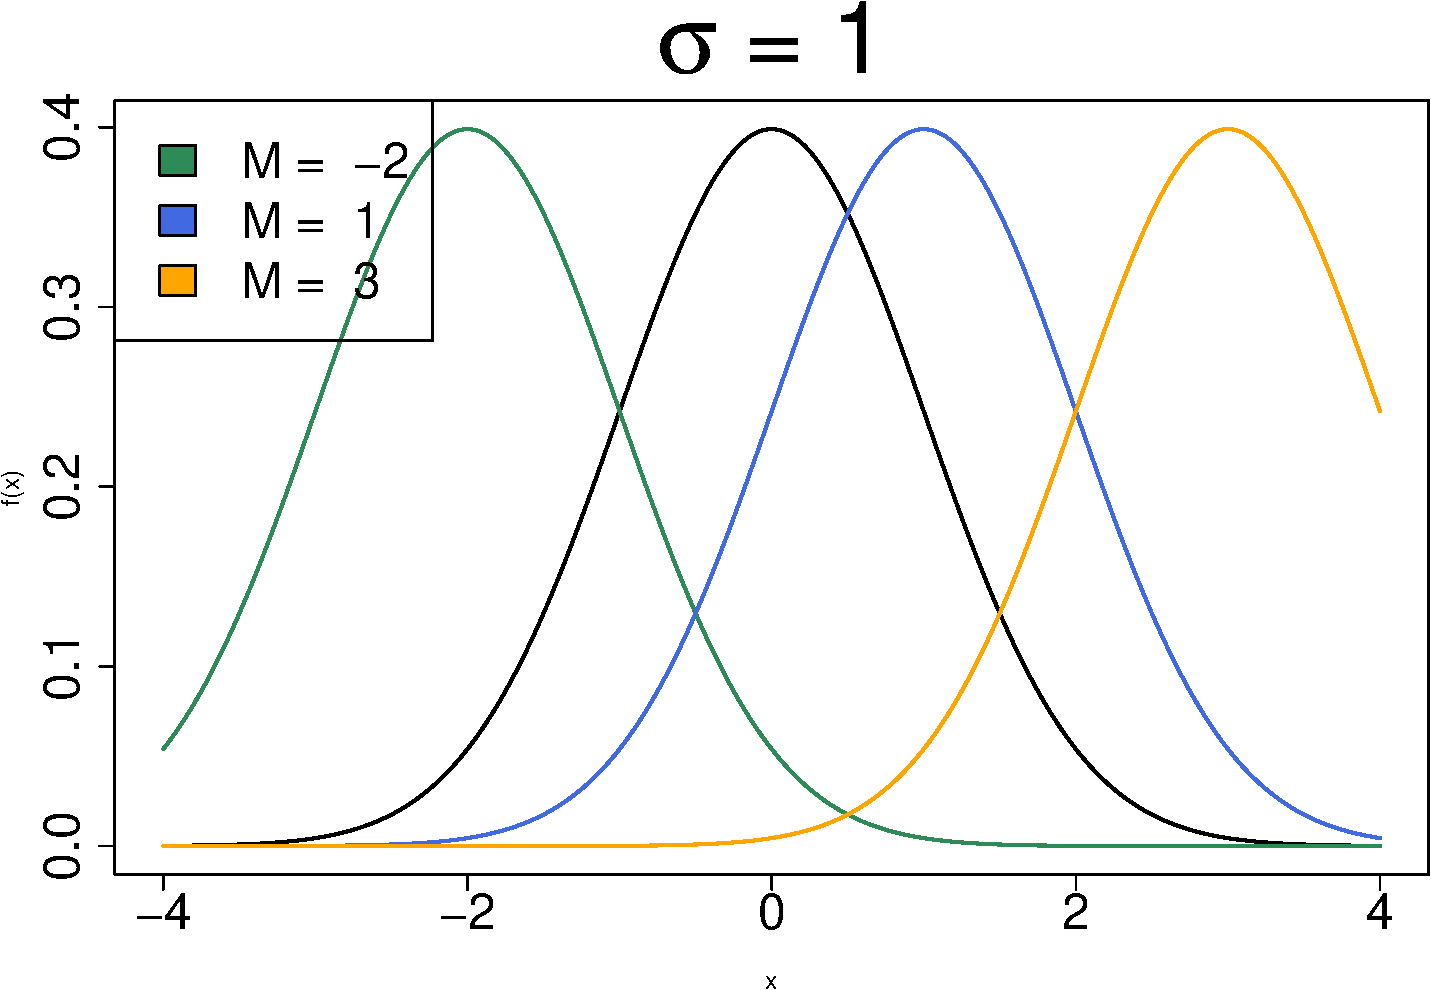
\includegraphics[keepaspectratio]{modulo4_files/figure-beamer/unnamed-chunk-13-1.pdf}}

}

\subcaption{Densità}

\end{figure}%

\end{minipage}%
%
\begin{minipage}{0.50\linewidth}

\begin{figure}[H]

{\centering \pandocbounded{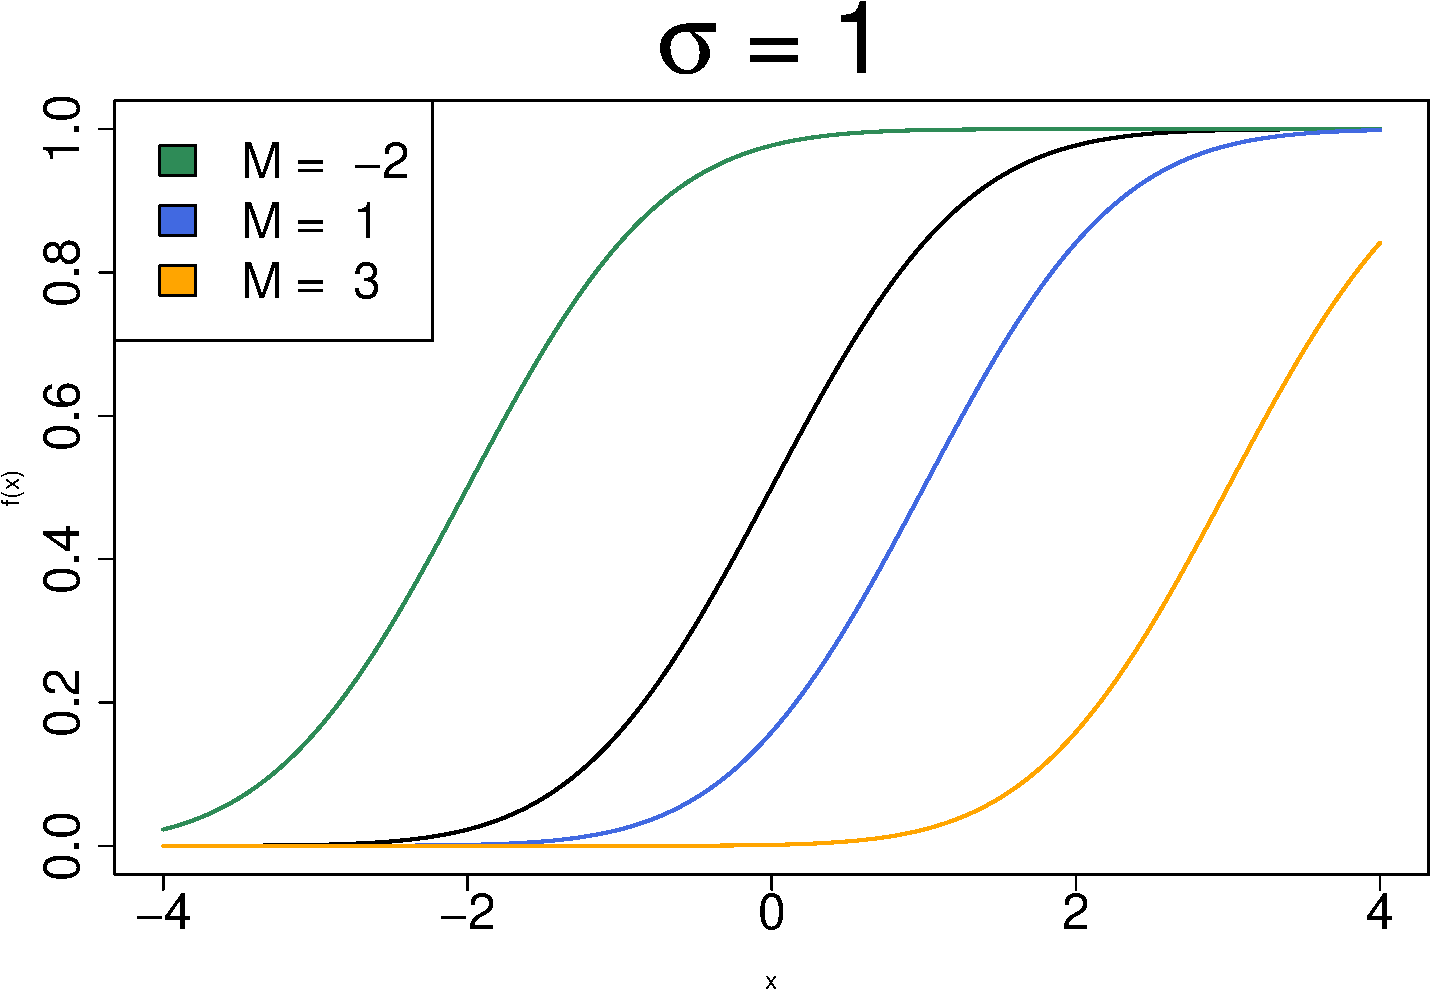
\includegraphics[keepaspectratio]{modulo4_files/figure-beamer/unnamed-chunk-13-2.pdf}}

}

\subcaption{Cumulata}

\end{figure}%

\end{minipage}%
\newline
\begin{minipage}{0.50\linewidth}
Stessa SD, media diversa\end{minipage}%

\end{figure}%
\end{frame}

\subsection{\texorpdfstring{\(t\) di
Student}{t di Student}}\label{t-di-student}

\begin{frame}{}
\phantomsection\label{section-21}
Definita da un unico parametro \(\theta = df\),
\(\Theta = (\mathbb{R}^+)\) (dove \(df = N-1\))

\begin{center}
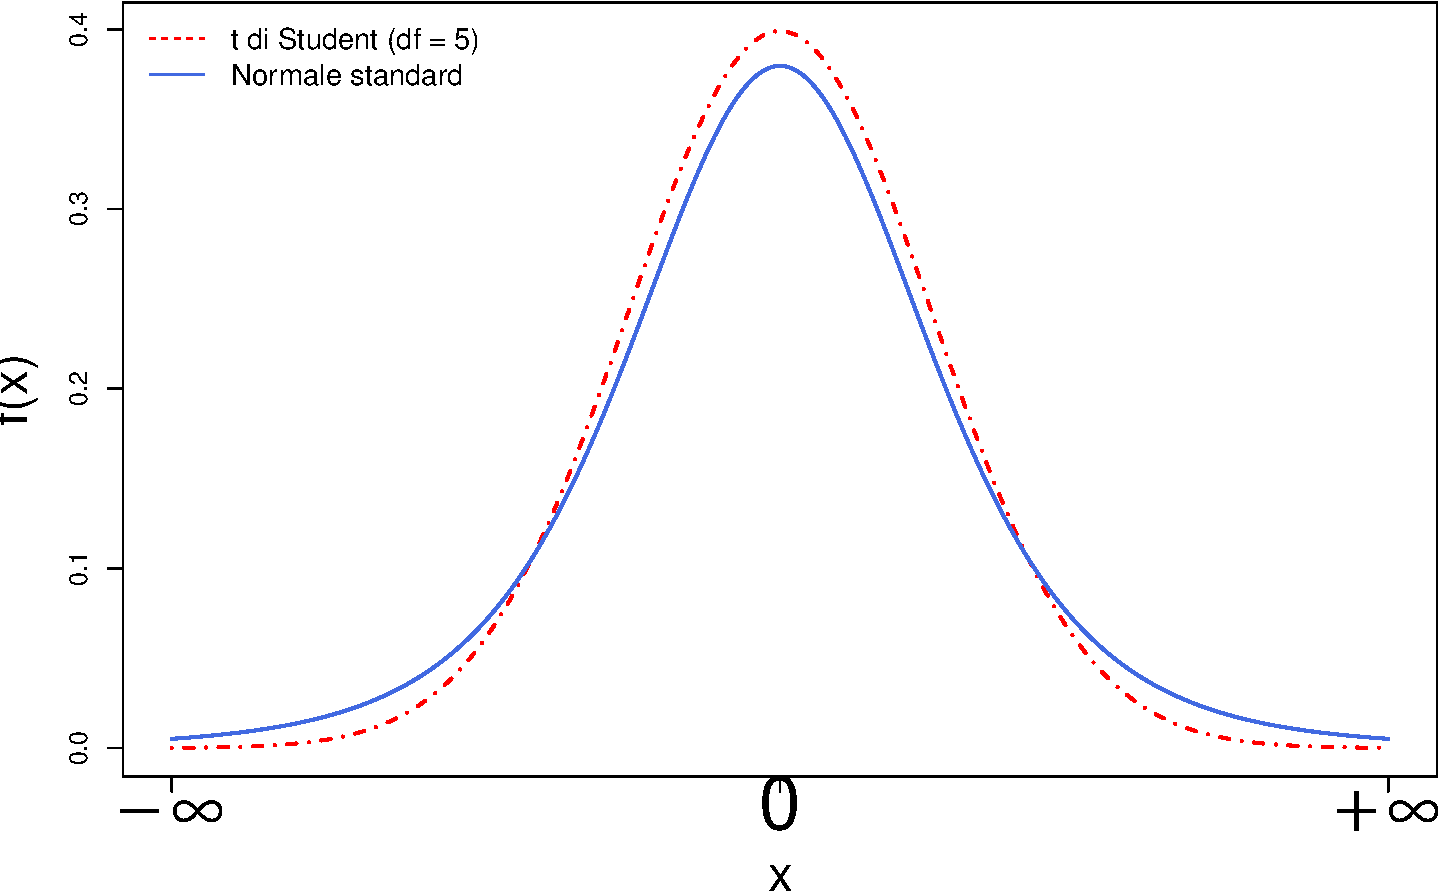
\includegraphics[width=0.7\linewidth,height=\textheight,keepaspectratio]{modulo4_files/figure-beamer/unnamed-chunk-14-1.pdf}
\end{center}
\end{frame}

\begin{frame}{}
\phantomsection\label{section-22}
\[\int_{-\infty}^{+\infty} f(t_v) dt = 1\]

\begin{center}
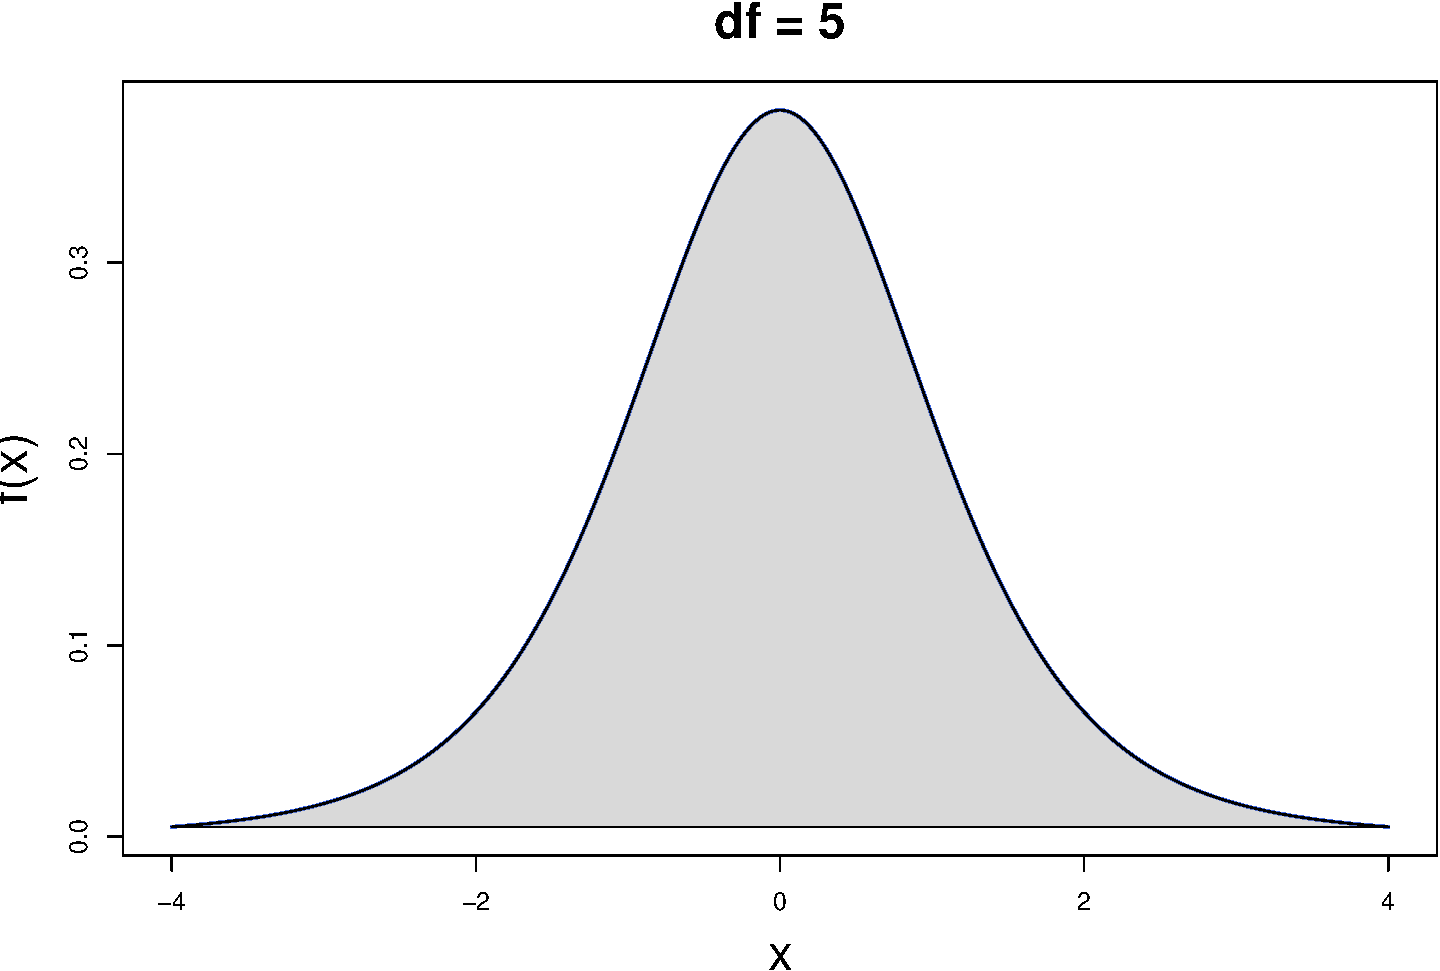
\includegraphics[width=0.7\linewidth,height=\textheight,keepaspectratio]{modulo4_files/figure-beamer/unnamed-chunk-15-1.pdf}
\end{center}
\end{frame}

\begin{frame}{}
\phantomsection\label{section-23}
\begin{figure}

\begin{minipage}{0.50\linewidth}

\begin{figure}[H]

{\centering \pandocbounded{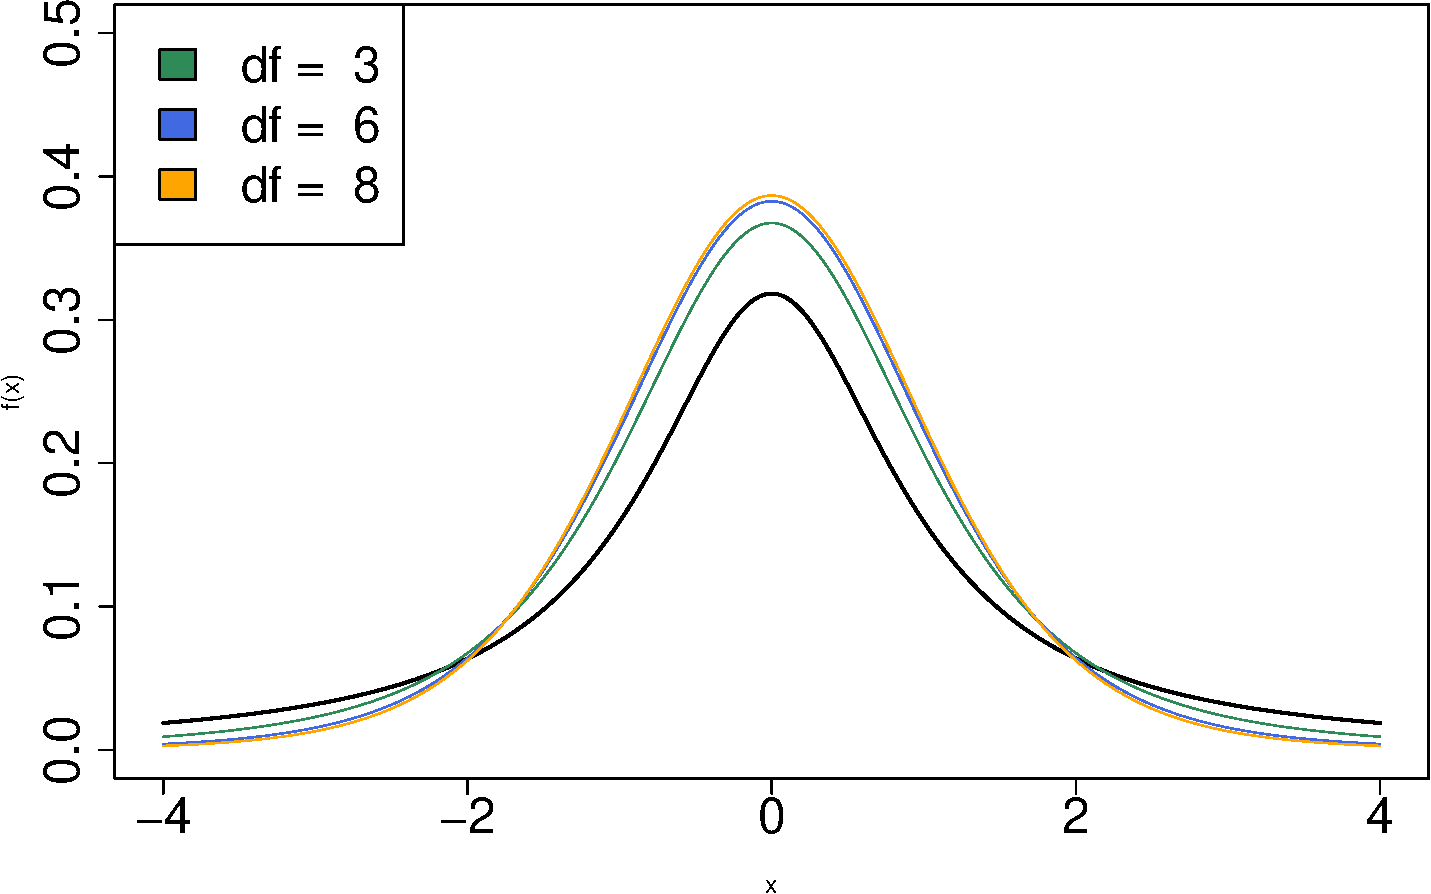
\includegraphics[keepaspectratio]{modulo4_files/figure-beamer/unnamed-chunk-16-1.pdf}}

}

\subcaption{Densità}

\end{figure}%

\end{minipage}%
%
\begin{minipage}{0.50\linewidth}

\begin{figure}[H]

{\centering \pandocbounded{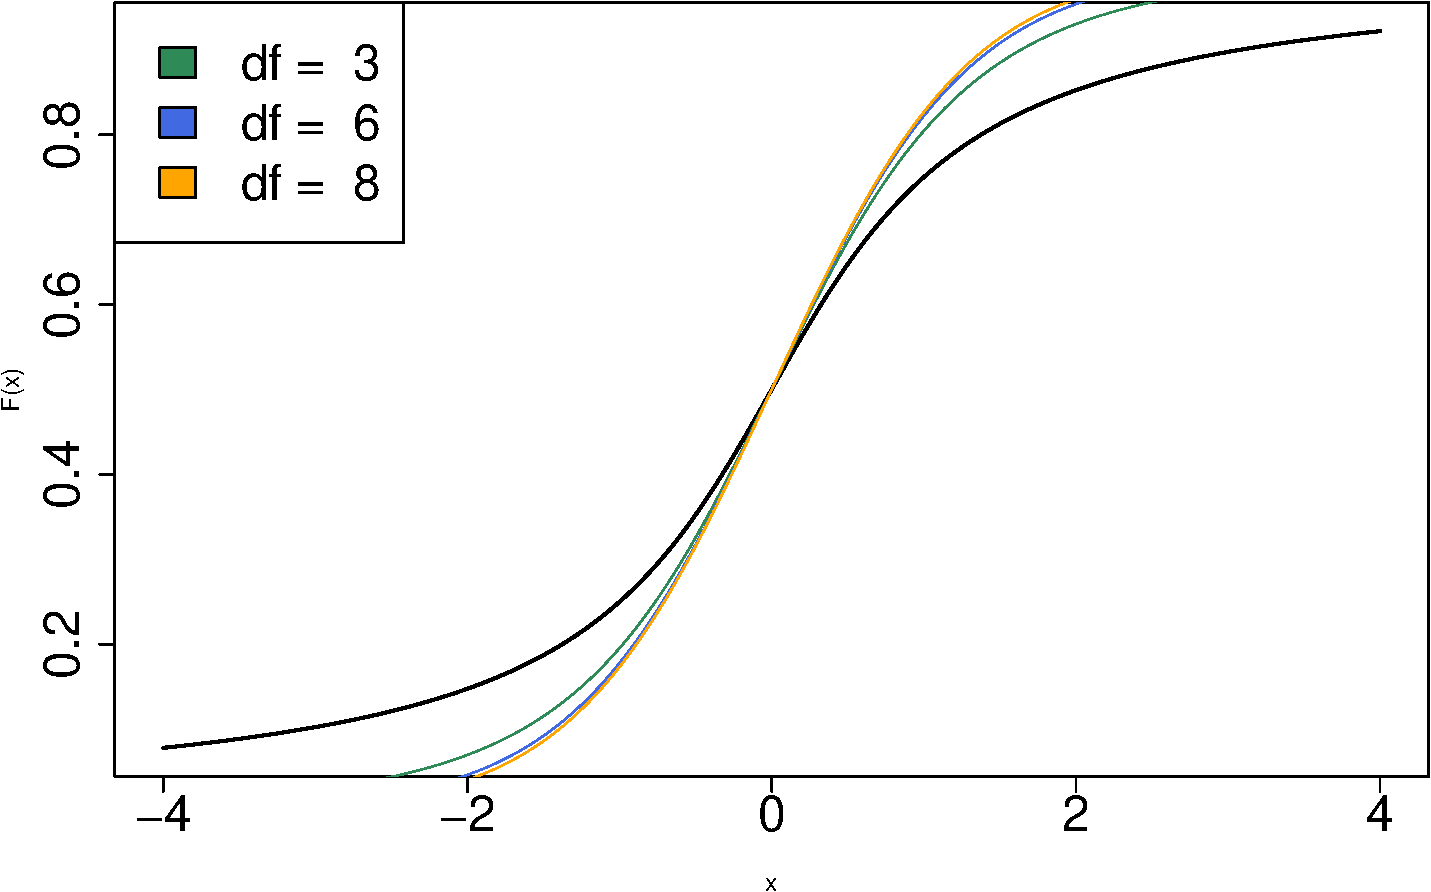
\includegraphics[keepaspectratio]{modulo4_files/figure-beamer/unnamed-chunk-16-2.pdf}}

}

\subcaption{Cumulata}

\end{figure}%

\end{minipage}%
\newline
\begin{minipage}{0.50\linewidth}
\(\theta = df\), \(\Theta = R^+\)\end{minipage}%

\end{figure}%
\end{frame}

\begin{frame}[fragile]{}
\phantomsection\label{section-24}
\begin{longtable}[]{@{}
  >{\raggedright\arraybackslash}p{(\linewidth - 2\tabcolsep) * \real{0.4348}}
  >{\raggedright\arraybackslash}p{(\linewidth - 2\tabcolsep) * \real{0.5652}}@{}}
\toprule\noalign{}
\begin{minipage}[b]{\linewidth}\raggedright
Funzione
\end{minipage} & \begin{minipage}[b]{\linewidth}\raggedright
Descrizione
\end{minipage} \\
\midrule\noalign{}
\endhead
\texttt{dt(x,\ df)} & Restituisce i \emph{valori di densità} associati
al vettore quantitativo \texttt{x} di una distribuzione t con gradi di
libertà (\texttt{df}). \\
\texttt{pt(x,\ df)} & Restituisce i \emph{valori di probabilità
cumulata} associati al vettore quantitativo \texttt{x}. \\
\texttt{qt(p,\ df)} & Restituisce i \emph{valori dei quantili} associati
al vettore di probabilità \texttt{p}. \\
\texttt{rt(n,\ df)} & Restituisce un vettore casuale di \texttt{n}
osservazioni indipendenti campionate da una distribuzione t di Student
con \texttt{df}. \\
\bottomrule\noalign{}
\end{longtable}
\end{frame}

\subsection{\texorpdfstring{Distribuzione
\(\chi^2\)}{Distribuzione \textbackslash chi\^{}2}}\label{distribuzione-chi2}

\begin{frame}{}
\phantomsection\label{section-25}
\begin{figure}

\begin{minipage}{0.50\linewidth}

\begin{figure}[H]

{\centering \pandocbounded{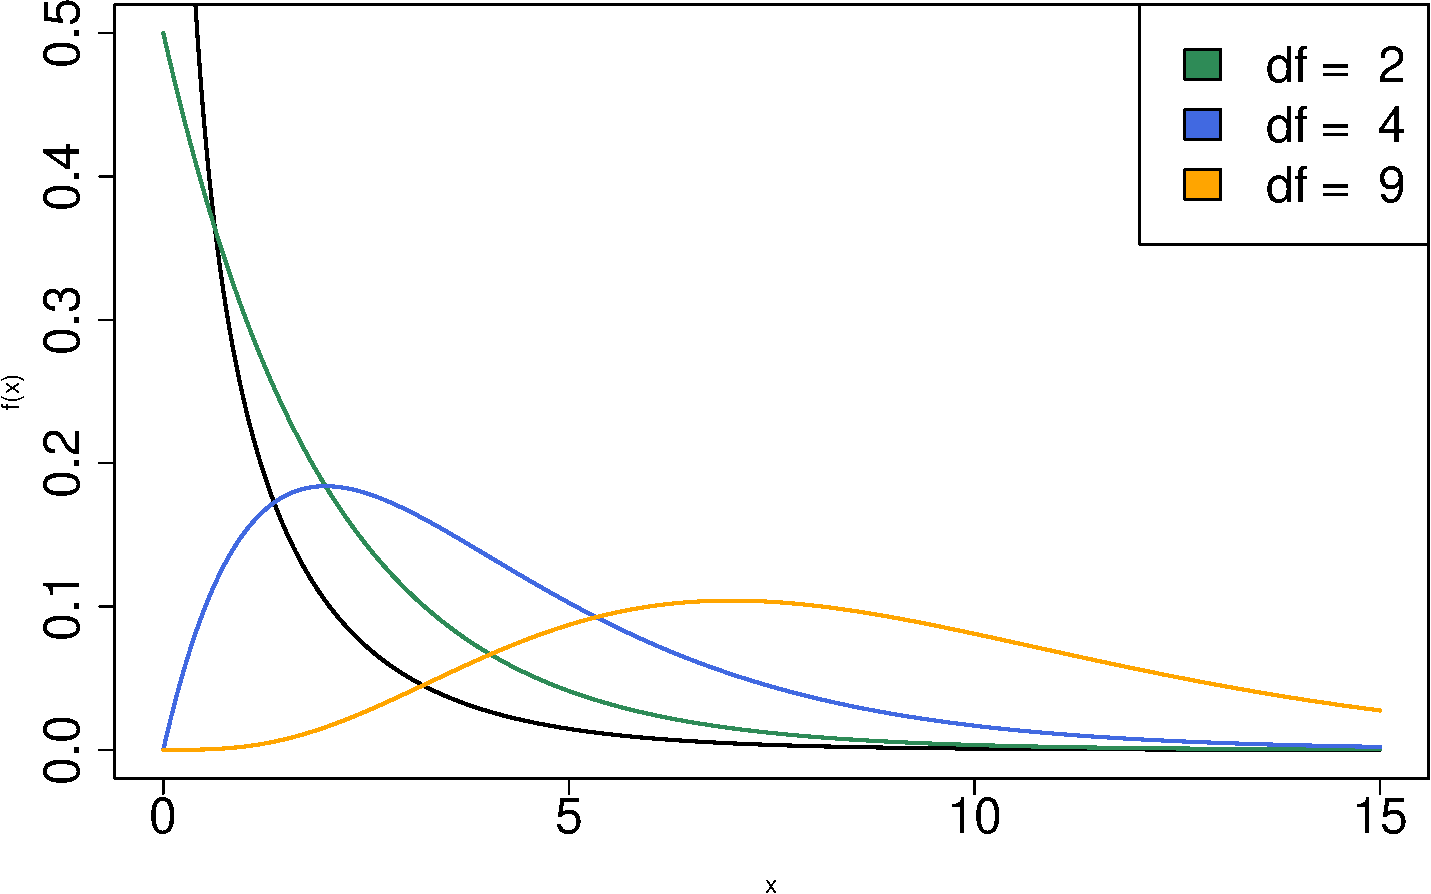
\includegraphics[keepaspectratio]{modulo4_files/figure-beamer/unnamed-chunk-17-1.pdf}}

}

\subcaption{Densità}

\end{figure}%

\end{minipage}%
%
\begin{minipage}{0.50\linewidth}

\begin{figure}[H]

{\centering \pandocbounded{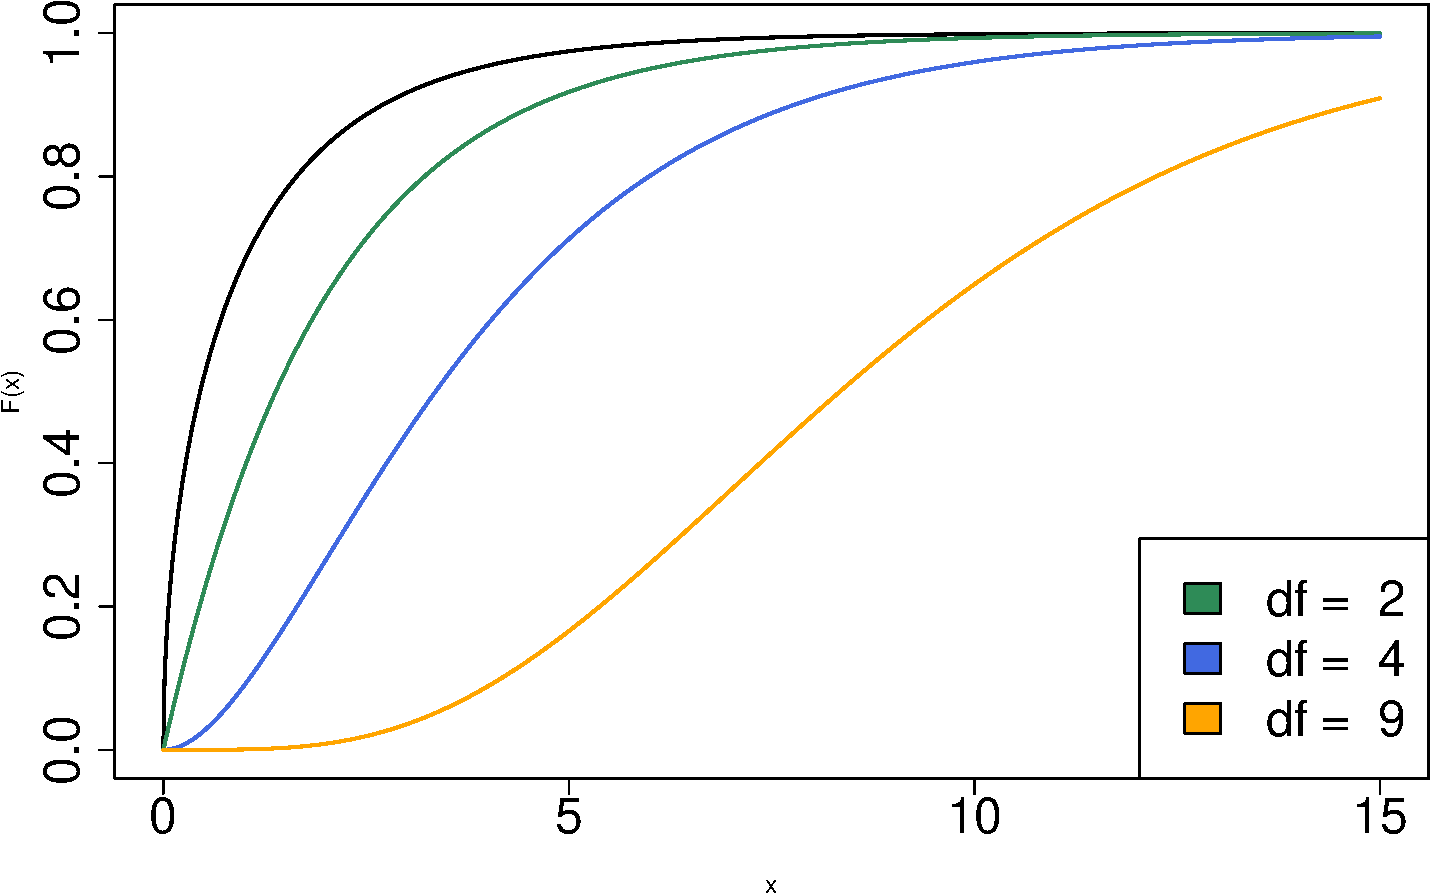
\includegraphics[keepaspectratio]{modulo4_files/figure-beamer/unnamed-chunk-17-2.pdf}}

}

\subcaption{Cumulata}

\end{figure}%

\end{minipage}%
\newline
\begin{minipage}{0.50\linewidth}
\(\theta = df\), \(\Theta = R^+\)\end{minipage}%

\end{figure}%
\end{frame}

\begin{frame}[fragile]{}
\phantomsection\label{section-26}
\begin{longtable}[]{@{}
  >{\raggedright\arraybackslash}p{(\linewidth - 2\tabcolsep) * \real{0.4348}}
  >{\raggedright\arraybackslash}p{(\linewidth - 2\tabcolsep) * \real{0.5652}}@{}}
\toprule\noalign{}
\begin{minipage}[b]{\linewidth}\raggedright
Funzione
\end{minipage} & \begin{minipage}[b]{\linewidth}\raggedright
Descrizione
\end{minipage} \\
\midrule\noalign{}
\endhead
\texttt{dchisq(x,\ df)} & Restituisce i \emph{valori di densità}
associati al vettore quantitativo \texttt{x} di una distribuzione
Chi-quadrato con gradi di libertà (\texttt{df}). \\
\texttt{pchisq(x,\ df)} & Restituisce i \emph{valori di probabilità
cumulata} associati al vettore quantitativo \texttt{x}. \\
\texttt{qchisq(p,\ df)} & Restituisce i \emph{valori dei quantili}
associati al vettore di probabilità \texttt{p}. \\
\texttt{rchisq(n,\ df)} & Restituisce un vettore casuale di \texttt{n}
osservazioni indipendenti campionate da una distribuzione chi-quadrato
con \texttt{df}. \\
\bottomrule\noalign{}
\end{longtable}
\end{frame}

\subsection{Altre distribuzioni
continue}\label{altre-distribuzioni-continue}

\begin{frame}[fragile]{}
\phantomsection\label{section-27}
\begin{tcolorbox}[enhanced jigsaw, arc=.35mm, opacityback=0, colback=white, coltitle=black, colframe=quarto-callout-tip-color-frame, rightrule=.15mm, bottomtitle=1mm, opacitybacktitle=0.6, titlerule=0mm, title={Esponenziale \texttt{exp}}, leftrule=.75mm, toprule=.15mm, toptitle=1mm, bottomrule=.15mm, colbacktitle=quarto-callout-tip-color!10!white, left=2mm, breakable]

\texttt{dexp(x,\ lambda)}, \texttt{pexp(x,\ lambda)},
\texttt{qexp(p,\ lambda)}, \texttt{rexp(n,\ lambda)}

\texttt{lambda} è il rate della distribuzione esponenziale

\end{tcolorbox}

\begin{tcolorbox}[enhanced jigsaw, arc=.35mm, opacityback=0, colback=white, coltitle=black, colframe=quarto-callout-tip-color-frame, rightrule=.15mm, bottomtitle=1mm, opacitybacktitle=0.6, titlerule=0mm, title={Uniforme \texttt{unif}}, leftrule=.75mm, toprule=.15mm, toptitle=1mm, bottomrule=.15mm, colbacktitle=quarto-callout-tip-color!10!white, left=2mm, breakable]

\texttt{dunif(x,\ min,\ max)}, \texttt{punif(x,\ min,\ max)},
\texttt{qunif(p,\ min,\ max)}, \texttt{runif(n,\ min,\ max)}

\texttt{min,\ max} valore minimo e massimo della distribuzione

\end{tcolorbox}
\end{frame}

\begin{frame}[fragile]{}
\phantomsection\label{section-28}
\begin{tcolorbox}[enhanced jigsaw, arc=.35mm, opacityback=0, colback=white, coltitle=black, colframe=quarto-callout-tip-color-frame, rightrule=.15mm, bottomtitle=1mm, opacitybacktitle=0.6, titlerule=0mm, title={Gamma \texttt{gamma}}, leftrule=.75mm, toprule=.15mm, toptitle=1mm, bottomrule=.15mm, colbacktitle=quarto-callout-tip-color!10!white, left=2mm, breakable]

\texttt{dgamma(x,\ shape,\ scale)}, \texttt{pgamma(x,\ shape,\ scale)},
\texttt{qgamma(p,\ shape,\ scale)}, \texttt{rgamma(n,\ shape,\ scale)}

\texttt{shape}: regola la forma della distribzuione, \texttt{scale}
regola la varianza

\end{tcolorbox}
\end{frame}




\end{document}
